\documentclass[10pt,a4paper]{article}
\usepackage[utf8]{inputenc}
\usepackage[english,russian]{babel}
\usepackage{cmap}
\usepackage[OT1]{fontenc}
\usepackage{amsmath}
\usepackage{amsfonts}
\usepackage{amssymb}
\usepackage{graphicx}
\usepackage{float}
\usepackage{wrapfig}
\usepackage{caption}
\DeclareCaptionLabelSeparator{dot}{. }
\captionsetup{justification=centering,labelsep=dot}
\graphicspath{{pictures/}}
\DeclareGraphicsExtensions{.pdf,.png,.jpg,.eps}
\begin{document}



\textbf{12 Разреженный обобщенный информационный фильтр}\\

\textbf{12.1	Введение}\\

В предыдущих двух главах были описаны противоположные реализации в спектре алгоритмов SLAM. Уже было замечено, что EKF SLAM построен как \textit{проактивный}. При каждом получении новой порции информации он реализует ее в виде вероятностного распределения, что вычислительно весьма затратно. Алгоритм GraphSLAM выполняется по другому и просто накапливает информацию. Принято считать такое накопление \textit{ленивым}: в момент получения данных GraphSLAM просто запоминает полученную информацию. Для превращения собранной информации в карту GraphSLAM выполняет вывод, который может быть осуществлён только после сбора всех данных, что делает GraphSLAM оффлайновым алгоритмом.

Возникает вопрос о возможности вывода \textit{онлайнового} алгоритма фильтра, который унаследовал бы эффективность информационного отображения. Это возможно, но лишь с рядом приближений. Разреженный обобщенный информационный фильтр (sparse extended information filter или SEIF), реализует информационное решение для проблемы онлайн SLAM. Так же, как и в EKF, SEIF интегрирует и удаляет прошлые положения робота, сохраняя лишь апостериорное распределение по текущему положению робота и карте. Но, так же, как GraphSLAM и, в отличие от EKF SLAM, SEIF поддерживает информационное выражение всей информации. В результате, такт обновления в SEIF становится ленивой операцией информационного сдвига, превосходящей проективное вероятностное обновление EKF. Поэтому SEIF можно считать наилучшим выбором, поскольку он запускается онлайн и вычислительно эффективен. 

Будучи онлайн алгоритмом, SEIF сохраняет оценку того же самого информационного вектора, что и EKF:\\

(12.1)
$$y_t=\left(\begin{array}{c}x_t\\m\\
\end{array} \right)$$

\begin{figure}[H]
	\center{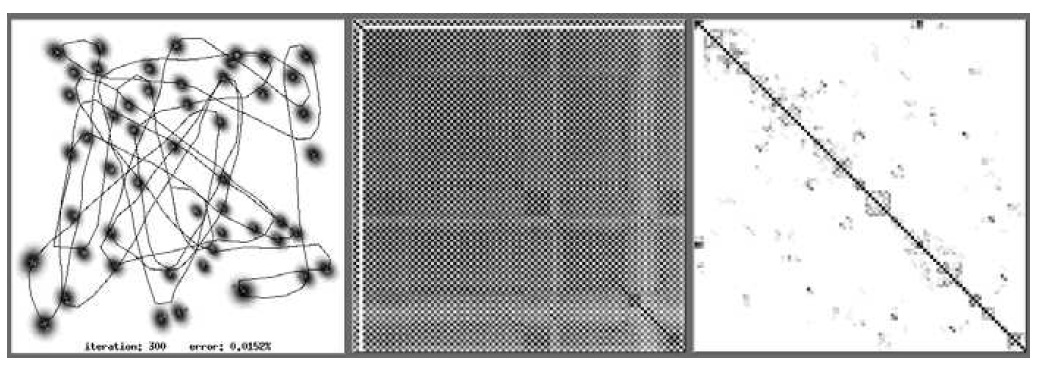
\includegraphics[width=1\linewidth]{121orig}}
	\caption{ ( Рис. 12.1 Причины использования информационного фильтра в онлайн SLAM. Слева: Проход робота в имитационной среде с 50 ориентирами. В центре: Матрица корреляции EKF, демонстрирующая сильную корреляцию между двумя любыми координатами ориентиров. Справа: нормализованная информационная матрица EKF изначально разрежена. Эта разреженность позволяет использовать алгоритм SLAM, который позволяет более эффективное обновление.) }
	\label{fig:121orig}
\end{figure}

Здесь $x_t$ – положение робота, а $m$ - карта. Апостериорная вероятность с известным соответствием задана в виде $p(y_t|z_{1:t}, u_{1:t}, c_{1:t})$.

Ключевая идея превращения GraphSLAM в алгоритм онлайн SLAM показана на Рис. 12.1. На рисунке показан результат работы алгоритма EKF SLAM в имитационной среде, где размещены 50 ориентиров. На левой врезке показан движущийся робот, а также вероятностная оценка местоположения для всех 50 точечных признаков. Главная информация, которая сохраняется в EKF SLAM - это ковариационная матрица различных оценок. Корреляция, которая является нормализованной ковариацией, показана на центральной врезке рисунка. По каждой из двух осей показано положение робота (местоположение и ориентация по направлению), а также двухмерное местоположение всех 50 ориентиров. Тёмные элементы сильно коррелированны. В главе, посвящённой EKF SLAM, уже обсуждалось, что в пределе координаты всех признаков становятся полностью коррелированными – отсюда и схожесть матрицы корреляции с шахматной доской.

На правой врезке Рис. 12.1 показана информационная матрица $\varOmega_t$, нормализованная так же, как матрица корреляции. Так же, как и в предыдущей главе, элементы этой нормализованной информационной матрицы можно воспринимать в виде ограничения или связи, которые ограничивают относительные положения пар признаков на карте. Чем темнее показанный элемент, тем сильнее связь. Как видно из рисунка, нормализованная информационная матрица выглядит разреженной. В ней преобладает небольшое количество сильных связей и имеется множество связей, значения которых при нормализации становятся практически равным нулю. 

\begin{figure}[H]
	\center{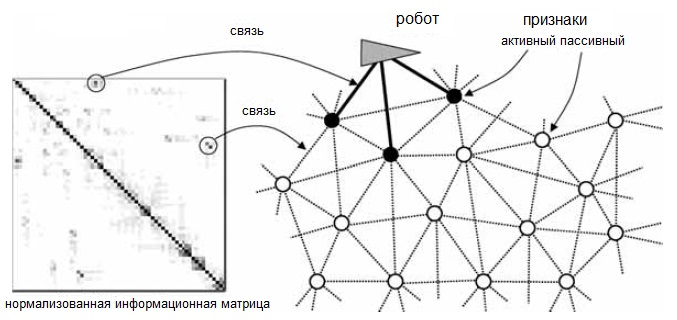
\includegraphics[width=1\linewidth]{122orig}}
	\caption{ ( Рис. 12.2 Иллюстрация сети признаков, сгенерированной нашим методом. Слева показана разреженная информационная матрица, а справа – карта, значения в которой связаны только ненулевые элементы информационной матрицы. Как упоминалось в тексте, тот факт, что не все признаки связаны, является ключевым структурным элементом задачи SLAM и основой нашего решения с постоянным временем.) }
	\label{fig:122orig}
\end{figure}

Сила каждой связи связана с расстоянием между соответствующими признаками, то есть сильные связи расположены только между близлежащими признаками. Чем дальше признаки друг от друга, тем слабее связь.

Эта концепция разреженности сильно отличается от описанной в предыдущей главе. Во-первых, существуют связи между парами признаков. В предыдущей главе такие связи не могли существовать. Во-вторых, сама разреженность лишь приблизительная. Фактически, хотя элементы нормализованной информационной матрицы ненулевые, но, практически все близки к нулю.\\

РАЗРЕЖЕННАЯ ИНФОРМАЦИОННАЯ МАТРИЦА\\

Алгоритм SEIF SLAM использует эту идею, сохраняя разреженную информационную матрицу, в которой только близлежащие признаки соединены ненулевым элементом.
Результирующая сетевая структура показана справа на Рис. 12.2, где кружки означают точечные признаки, а пунктирные дуги – связи, изображённые в информационной матрице слева. На этой схеме также показан робот, который связан лишь с небольшим числом признаков.\\

АКТИВНЫЕ ПРИЗНАКИ\\

Эти признаки называются активными и изображены чёрным цветом. Хранение разреженной информационной матрицы требует объёма памяти, линейно зависящего от количества признаков на карте. Более важным является возможность выполнить все важные обновления SEIF SLAM за одинаковое время, независимо от количества признаков на карте. Этот результат достаточно нетривиален, поскольку наивная реализация обновления движения в информационных фильтрах, как указано в Таблице 3.6 на странице 76  ???, требует обращения всей информационной матрицы.

SEIF  - это онлайн алгоритм SLAM, сохраняющий такую разреженную информационную матрицу, время выполнения всех тактов обновления которой не зависит от размера карты для случая известной ассоциации данных, и зависит логарифмически, если необходимо выполнять поиск ассоциаций. Это делает SEIF первым эффективным онлайновым SLAM алгоритмом, приведённом в книге.\\

\textbf{12.2	Интуитивное описание}\\

Начнём с интуитивного описания обновления SEIF, используя графические иллюстрации. Обновление SEIF состоит из 4 действий: обновление движения, обновление измерения, разреживание и обновление состояния.

Алгоритм начинается с шага обновления измерения, показанного на Рис. 12.3. На обеих врезках показана информационная матрица, сохраняемая SEIF, а также граф, определённый информационными связями. Так же, как и в GraphSLAM, обнаружение признака $m_1$ заставляет алгоритм SEIF обновить недиагональный элемент информационной матрицы, соединяющий оценку положения робота $x_t$ с наблюдаемым признаком $m_1$. Это показано на схеме слева на Рис. 12.3a.

Обнаружение признака $m_2$ приводит к обновлению элементов информационной матрицы, соединяющих положение робота $x_t$ и признак $m_2$, как показано на Рис. 12.3b. Как будет показано далее, каждому из этих обновлений соответствует локальное добавление в информационную матрицу и информационный вектор. В обоих случаях (и для информационной матрицы, и для вектора), эти добавления затрагивают только связи между переменной положения робота и наблюдаемым признаком. Так же, как в GraphSLAM, вычислительная сложность учёта измерения в SEIF не зависит от размера карты.

Обновление движение, однако, отличается от GraphSLAM, поскольку SEIF является фильтром и как показано на Рис. 12.4, отсекает оценки прошлых положений. Здесь происходит смена положения робота – на Рис. 12.4a показано информационное состояние до перемещения, а на Рис. 12.4b – после передвижения, соответственно. Движение влияет на информационное состояние в нескольких аспектах. Во-первых, ослабляется связь между положением робота и признаками $m_1$, $m_2$. Это является результатом привнесения движением робота дополнительной неопределённости, поскольку теряется информация о местонахождении робота относительно карты. Однако, потеря этой информации неполная и её часть проецирована в виде связи между признаками. Это информационный сдвиг происходит потому, что, несмотря на потерю информации о положении робота, информация об относительном местоположении признаков на карте сохранилась. Там, где эти признаки были связаны опосредовано через положение робота, после шага обновления они становятся связаны напрямую.

\begin{figure}[H]
	\center{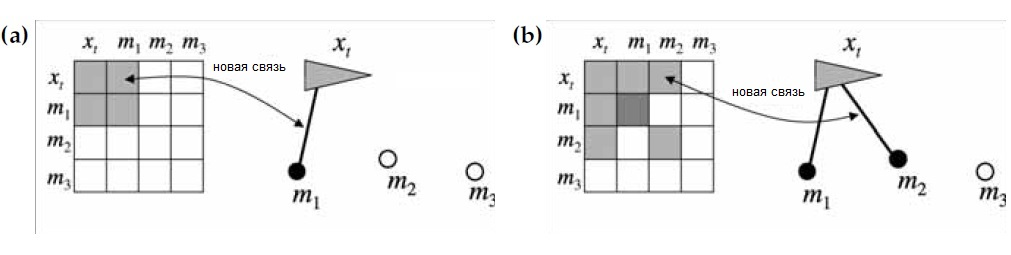
\includegraphics[width=1\linewidth]{123orig}}
	\caption{ ( Рис. 12.3 Воздействие измерений на информационную матрицу и связанную с ней сеть признаков: Наблюдение $m_1$ вызывает изменение элементов $\varOmega_{x_t,m_1}$  в информационной матрице (a).  Аналогично, наблюдение $m_2$ влияет на $\varOmega_{x_t,m_2}$ (b).) }
	\label{fig:123orig}
\end{figure}

\begin{figure}[H]
	\center{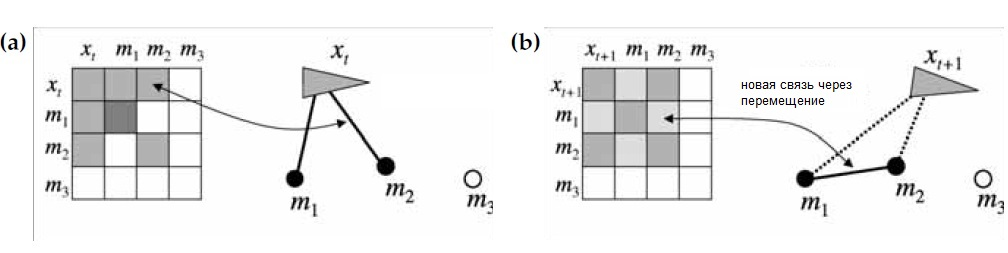
\includegraphics[width=1\linewidth]{124orig}}
	\caption{ ( Рис. 12.4 Воздействие движения на информационную матрицу и связанную с ней сеть признаков: до перемещения (a) и  после движения (b). Если движение не детерминировано, обновление движения образует новые связи (или усиливает существующие) между любыми двумя активными признаками, при этом связи между роботом и этими признаками ослабляются. На этом шаге образуются связи между парами признаков.) }
	\label{fig:124orig}
\end{figure}

\begin{figure}[H]
	\center{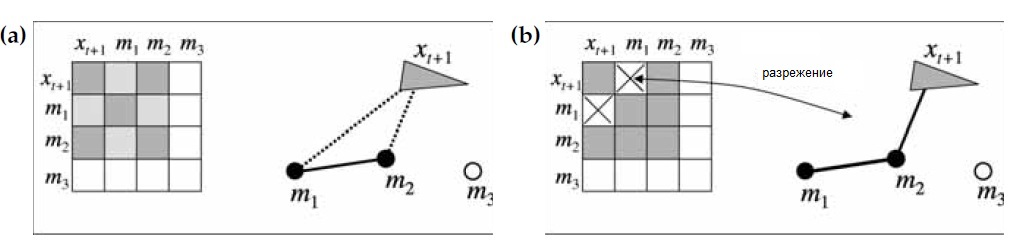
\includegraphics[width=1\linewidth]{125orig}}
	\caption{ ( Рис. 12.5 Разрежение: признак деактивируется уничтожением его связи с роботом. Для компенсации потери связи в информационном состоянии обновляются связи между активными признаками и/или роботом. Время выполнения всей операции постоянно. ) }
	\label{fig:125orig}
\end{figure}

Смещение информации от связи с роботом к связи между признаками является ключевым элементом SEIF. Это прямое следствие использования информационного представления в виде фильтра для задачи онлайн SLAM. При вычёркивании переменные прошлых положений робота связи с ними теряются, но заново проецируются на связи между признаками в информационной матрице. В этом состоит отличие от алгоритма GraphSLAM, обсуждаемого в предыдущей главе, в котором новые связи между парами признаков на карте не образуются никогда.

Чтобы между парой признаков образовалась новая связь, перед обновлением они оба должны быть активными, поскольку элементы соответствия, связывающие их с положением робота в информационной матрице, должны быть ненулевыми. Это показано на Рис. 12.4: Связь между признаками образуется только между $m_1$ и $m_2$. Неактивный признак $m_3$ остаётся незатронутым. Это подразумевает, что, управляя количеством активных ориентиров в произвольный момент времени, возможно управлять вычислительной сложностью обновления движения и количеством связей в информационной матрице. Если количество активных связей остаётся достаточно малым, вычислительная сложность обновления движения тоже будет небольшой, как и количество ненулевых элементов связей между ориентирами в информационной матрице.\\

РАЗРЕЖЕНИЕ\\

На этом шаге алгоритм SEIF выполняет \textit{разрежение}, как показано на Рис. 12.5. Разрежение включает удаление связи между роботом и активным признаком, эффективно превращая активный признак в пассивный. В SEIF это удаление дуги ведёт к перераспределению информации на соседние связи, в частности, между активными признаками и положением робота. Требуемое для разрежения время не зависит от размера карты. Однако, поскольку это операция приближения, происходит потеря информации в апостериорной вероятности. Преимуществом такого приближения является вносимая разреженность, что позволяет эффективно выполнять обновление фильтра.

Существует ещё один, последний шаг выполнения алгоритма SEIF, не показанный на рисунках. На этом шаге выполняется распространение средней оценки по графу. Как уже обсуждалось в Главе 3, в обобщённом информационном фильтре для выполнения линеаризации моделей движения и измерения требуется оценка состояния $\mu_t$. В SEIF для шага разрежения также требуется оценка состояния.\\

АЛГОРИТМ РЕЛАКСАЦИИ\\

Строго говоря, можно восстановить оценку состояния через равенство $\mu=\varOmega^{-1}\xi$, где $\varOmega$ - информационный вектор, а $\xi$ - информационное состояние. Однако, это потребует решения задачи вывода, слишком большой для обработки ее на каждом такте времени. В SEIF этот шаг выполняется с помощью алгоритма релаксации, распространяющего оценки состояния в информационном графе. Каждая локальная оценка состояния обновляется на основании наилучших оценок соседних узлов информационного графа. Этот алгоритм релаксации сходится к точному значению среднего $\mu$. Поскольку информационный вид в SEIF разрежённый, каждое такое обновление выполняется за постоянное время, хотя и с допущением необходимости большого количества  таких обновлений для получения хороших результатов. Для поддержания вычислительной сложности, независимой от размера пространства состояний, в SEIF при каждой итерации выполняется фиксированное количество таких обновлений. Результирующий вектор состояния является приближенным и используется вместо правильной оценки среднего на всех шагах обновления.\\  

\textbf{12.3	Алгоритм SEIF SLAM} \\

Внешний цикл обновления SEIF показан в Таблице 12.1. Алгоритм принимает на вход информационную матрицу $\varOmega_{t-1}$, информационный вектор $\xi_{t-1}$ и оценку состояния $\mu_{t-1}$.   Также принимаются измерение $z_t$, управляющее воздействие $u_t$ и вектор соответствия $c_t$. Выход алгоритма \textbf{SEIF\_SLAM\_known\_correspondences} даёт новую оценку состояния, выраженную информационной матрицей $\varOmega_t$ и информационным вектором $\xi_t$, а также улучшенную оценку $\mu_t$.

Как указано в Таблице 12.1, обновление SEIF происходит за четыре основных шага. Обновление движения в Таблице 12.2 учитывает управляющее воздействие $u_t$ в оценке фильтра с помощью ряда вычислительно эффективных операций. Например, единственными модифицируемыми при этом обновлении компонентами информационного вектора/матрицы являются положение робота и активные признаки. Обновление измерения в Таблице 12.3 учитывает вектор измерения $z_t$ с известным соответствием $c_t$. Этот шаг выполняется локально, так же, как обновление движения, то есть обновляются только информационные значения положения робота и наблюдаемых признаков на карте. Шаг разрежения, показанный в Таблице 12.4, является приближением: он удаляет активные признаки, преобразуя соответствующим образом информационную матрицу и информационный вектор. Этот шаг также вычислительно эффективен, поскольку затрагивает только связи между роботом и активными ориентирами. Наконец, обновление оценки состояния в Таблице 12.5, использует смягченный метод покоординатного спуска для восстановления оценки состояния $\mu_t$. На этом шаге вновь используется разреженность SEIF, благодаря которой при каждом инкрементном обновлении необходимо обратиться лишь к небольшому числу других элементов вектора состояний. 

Весь совокупный цикл обновления SEIF выполняется за постоянное время, которое не зависит от размера карты. Это является прямой противоположностью другого обсуждаемого алгоритма SLAM—EKF, в котором для каждого обновления требуется время, квадратично зависящее от размера карты. 

\begin{table}[H]
\begin{center}
\begin{tabular}{|l|}
\hline
{}\\
1:\textbf{ Algorithm SEIF\_SLAM\_known\_correspondences}$(\xi_{t-1},\varOmega_{t-1},$\\
\hspace{95mm}$\mu_{t-1},u_t,z_t,c_t)$:\\
2:\hspace{5mm}$\bar{\xi}_t,\bar{\varOmega}_t,\bar{\mu}_t=\textbf{SEIF\_motion\_update}(\xi_{t-1},\varOmega_{t-1},\mu_{t-1},u_t)$\\
3:\hspace{5mm}$\mu_t=\textbf{SEIF\_update\_state\_estimate}(\bar{\xi}_t,\bar{\varOmega}_t,\bar{\mu}_t)$\\
4:\hspace{5mm}$\xi_t,\varOmega_t=\textbf{SEIF\_measurement\_update}(\bar{\xi}_t,\bar{\varOmega}_t,\mu_t,z_t,c_t)$\\
5:\hspace{5mm}$\bar{\xi}_t,\bar{\varOmega}_t=\textbf{SEIF\_sparsification}(\xi_t,\varOmega_t)$\\
6:\hspace{5mm}$\textit{return}\,\,\bar{\xi}_t,\bar{\varOmega}_t,\mu_t$\\
{}\\
\hline
\end{tabular}
\caption{(Таблица 12.1 Алгоритм разреженного обобщённого информационного фильтра для задачи SLAM с известной ассоциацией данных.)}
\end{center}
\end{table}

\begin{table}[H]
\begin{center}
\begin{tabular}{|l|}
\hline
{}\\
1:\textbf{ Algorithm SEIF\_motion\_update}$(\xi_{t-1},\varOmega_{t-1},\mu_{t-1},u_t):\qquad$\\
2:\hspace{5mm}$F_x=\left(\begin{array}{cccc}1&0&0&0...0\\
0&1&0&0...0\\
0&0&1&\underbrace{0...0}_{3N}\\
\end{array} \right)$\\
3:\hspace{5mm}$\delta=\left(\begin{array}{c}
-\frac{v_t}{\omega_t}\sin\mu_{t-1,\theta}+\frac{v_t}{\omega_t}\sin(\mu_{t-1,\theta}+\omega_t\varDelta t)\\
\frac{v_t}{\omega_t}\cos\mu_{t-1,\theta}-\frac{v_t}{\omega_t}\cos(\mu_{t-1,\theta}+\omega_t\varDelta t)\\
\omega_t\varDelta t\\
\end{array} \right)$\\
4:\hspace{5mm}$\varDelta=\left(\begin{array}{ccc}
0&0&\frac{v_t}{\omega_t}\cos\mu_{t-1,\theta}-\frac{v_t}{\omega_t}\cos(\mu_{t-1,\theta}+\omega_t\varDelta t)\\
0&0&\frac{v_t}{\omega_t}\sin\mu_{t-1,\theta}-\frac{v_t}{\omega_t}\sin(\mu_{t-1,\theta}+\omega_t\varDelta t)\\
0&0&0\\
\end{array} \right)$\\
5:\hspace{5mm}$\varPsi_t=F_x^T[(I+\varDelta)^{-1}-I]F_x$\\
6:\hspace{5mm}$\lambda_t=\varPsi_t^T\varOmega_{t-1}+\varOmega_{t-1}\varPsi_t+\varPsi_t^T\varOmega_{t-1}\varPsi_t$\\
7:\hspace{5mm}$\varPhi_t=\varOmega_{t-1}+\lambda_t$\\
8:\hspace{5mm}$\kappa_t=\varPhi_tF_x^T(R_t^{-1}+F_x\varPhi_tF_x^T)^{-1}F_x\varPhi_t$\\
9:\hspace{5mm}$\bar{\varOmega}_t=\varPhi_t-\kappa_t$\\
10:\hspace{4mm}$\bar{\xi}_t=\xi_{t-1}+(\lambda_t-\kappa_t)\mu_{t-1}+\bar{\varOmega}_tF_x^T\delta_t$\\
11:\hspace{4mm}$\bar{\mu}_t=\mu_{t-1}+F_x^T\delta$\\
12:\hspace{4mm}$\textit{return}\,\,\bar{\xi}_t,\bar{\varOmega}_t,\bar{\mu}_t$\\
{}\\
\hline
\end{tabular}
\caption{(Таблица 12.2    Обновление движения в SEIF.)}
\end{center}
\end{table}

\begin{table}[H]
\begin{center}
\begin{tabular}{|l|}
\hline
{}\\
1:\textbf{ Algorithm SEIF\_measurement\_update}$(\bar{\xi}_t,\bar{\varOmega}_t,\mu_t,z_t,c_t):\qquad$\\
2:\hspace{5mm}$Q_t=\left(\begin{array}{ccc}
\sigma_r&0&0\\
0&\sigma_\phi&0\\
0&0&\sigma_s\\
\end{array} \right)$\\
3:\hspace{5mm}$\textit{для всех наблюдаемых признаков}\,z_t^i=(r_t^i\,\,\phi_t^i\,\,s_t^i)^T\,\textit{do}$\\
4:\hspace{10mm}$j=c_t^i$\\
5:\hspace{10mm}$\textit{если ориентир j никогда не наблюдался}$\\
6:\hspace{15mm}$\left(\begin{array}{c}
\mu_{j,x}\\
\mu_{j,y}\\
\mu_{j,s}\\
\end{array} \right)=\left(\begin{array}{c}
\mu_{t,x}\\
\mu_{t,y}\\
s_t^i\\
\end{array} \right)+r_t^i\left(\begin{array}{c}
\cos(\phi_t^i+\mu_{t,\theta})\\
\sin(\phi_t^i+\mu_{t,\theta})\\
0\\
\end{array} \right)$\\
7:\hspace{10mm}$\textit{endif}$\\
8:\hspace{10mm}$\delta=\left(\begin{array}{c}\delta_x\\\delta_y\\\end{array} \right)=\left(\begin{array}{c}
\mu_{j,x}-\mu_{t,x}\\
\mu_{j,y}-\mu_{t,y}\\
\end{array} \right)$\\
9:\hspace{10mm}$q=\delta^T\delta$\\
10:\hspace{9mm}$\hat{z}_t^i=\left(\begin{array}{c}
\sqrt{q}\\
\text{atan2}(\delta_y,\delta_x)-\mu_{t,\theta}\\
\mu_{j,s}\\
\end{array} \right)$\\
11:\hspace{9mm}$H_t^i=\frac{1}{q}\left(\begin{array}{cccccccc}
\sqrt{q}\delta_x&-\sqrt{q}\delta_y&0&0...0&-\sqrt{q}\delta_x&\sqrt{q}\delta_y&0&0...0\\
\delta_y&\delta_x&-1&0...0&-\delta_y&-\delta_x&0&0...0\\
0&0&0&\underbrace{0...0}_{3j-3}&0&0&1&\underbrace{0...0}_{3j}\\
\end{array} \right)$\\
12:\hspace{4mm}$\textit{endfor}$\\
13:\hspace{4mm}$\xi_t=\bar{\xi}_t+\varSigma_iH_t^{iT}Q_t^{-1}[z_t^i-\hat{z}_t^i-H_t^i\mu_t]$\\
14:\hspace{4mm}$\varOmega_t=\bar{\varOmega}_t+\varSigma_iH_t^{iT}Q_t^{-1}H_t^i$\\
15:\hspace{4mm}$\textit{return}\,\,\xi_t,\varOmega_t$\\
{}\\
\hline
\end{tabular}
\caption{(Таблица 12.3    Обновление измерения в SEIF.)}
\end{center}
\end{table}

\begin{table}[H]
\begin{center}
\begin{tabular}{|l|}
\hline
{}\\
1:\textbf{ Algorithm SEIF\_sparsification}$(\xi_t,\varOmega_t):\qquad\qquad\qquad\qquad$\\
2:\hspace{5mm}$\textit{определить}\,F_{m_0},F_{x,m_0},F_x\,\textit{как проекционные матрицы}$\\
$\hspace{25mm}\textit{от}\,y_t\,\textit{до}\,m_0,\{x,m_0\}\textit{и}\,x,\,\textit{соответственно}$\\
3:\hspace{5mm}$\bar{\varOmega}_t=\varOmega_t-\varOmega_t^0F_{m_0}(F_{m_0}^T\varOmega_t^0F_{m_0})^{-1}F_{m_0}^T\varOmega_t^0$\\
$\hspace{25mm}+\varOmega_t^0F_{x,m_0}(F_{x,m_0}^T\varOmega_t^0F_{x,m_0})^{-1}F_{x,m_0}^T\varOmega_t^0$\\
$2:\hspace{25mm}-\varOmega_tF_x(F_x^T\varOmega_tF_x)^{-1}F_x^T\varOmega_t$\\
4:\hspace{5mm}$\bar{\xi}_t=\xi_t+\mu_t(\bar{\varOmega}_t-\varOmega_t)$\\
5:\hspace{5mm}$\textit{return}\,\,\bar{\xi}_t,\bar{\varOmega}_t$\\
{}\\
\hline
\end{tabular}
\caption{(Таблица 12.4    Шаг разрежения в SEIF.)}
\end{center}
\end{table}

\begin{table}[H]
\begin{center}
\begin{tabular}{|l|}
\hline
{}\\
1:\textbf{ Algorithm SEIF\_update\_state\_estimate}$(\bar{\xi}_t,\bar{\varOmega}_t,\bar{\mu}_t):\qquad\qquad$\\
2:\hspace{5mm}$\textit{для малого набора признаков карт }\,m_i\,\textit{do}$\\
3:\hspace{10mm}$F_i=\left(\begin{array}{cccc}
0...0&1&0&0...0\\\underbrace{0...0}_{2(N-i)}&0&1&\underbrace{0...0}_{2(i-1)x}\end{array} \right)$\\
4:\hspace{10mm}$\mu_{i,t}=(F_i\varOmega_tF_i^T)^{-1}F_i[\xi_t-\varOmega_t\bar{\mu}_t+\varOmega_tF_i^TF_i\bar{\mu}_t]$\\
5:\hspace{5mm}$\textit{endfor}$\\
6:\hspace{5mm}$\textit{для всех остальных признаков карты }\,m_i\,\textit{do}$\\
7:\hspace{10mm}$\mu_{i,t}=\bar{\mu}_{i,t}$\\
8:\hspace{5mm}$\textit{endfor}$\\
9:\hspace{5mm}$F_x=\left(\begin{array}{cccc}
1&0&0&0...0\\
0&1&0&0...0\\
0&0&1&\underbrace{0...0}_{3N}\end{array} \right)$\\
10:\hspace{4mm}$\mu_{x,t}=(F_x\varOmega_tF_x^T)^{-1}F_x[\xi_t-\varOmega_t\bar{\mu}_t+\varOmega_tF_x^TF_x\bar{\mu}_t]$\\
11:\hspace{4mm}$\textit{return}\,\mu_t$\\
{}\\
\hline
\end{tabular}
\caption{(Таблица 12.5 Шаг смягчённого обновления состояния в SEIF затрагивает небольшое количество оценок состояния.)}
\end{center}
\end{table}

SLAM С ПОСТОЯННЫМ ВРЕМЕНЕМ\\

Однако, такое предположение о “\textit{SLAM с постоянным временем}” следует воспринимать с некоторым скепсисом, поскольку восстановление оценок состояния в средах с большими циклами является вычислительной проблемой, для которой пока не существует решений, линейно зависящих от времени.

\textbf{12.4	Математический вывод SEIF}\\

\textbf{12.4.1	Обновление движения}\\

Обновление движения в SEIF обрабатывает управляющее воздействие $u_t$ путём преобразования информационной матрицы $\varOmega_{t-1}$ и информационного вектора $\xi_{t-1}$ в новую матрицу $\bar{\varOmega}_t$ и вектор $\bar{\xi}_t$.  Как обычно в нашей записи, черта указывает, что в этом прогнозе учитывается лишь управление, а измерение в расчёт не принимается.

Обновление движения в SEIF использует разреженность информационной матрицы, что позволяет выполнять его за время, не зависящее от размера карты $n$. Этот вывод лучше всего начать с соответствующей формулы для EKF. Начнём с алгоритма \textbf{EKF\_SLAM\_known\_correspondences} в Таблице 10.1 на странице 314 ???. Обновление движение происходит в строках 3 и 5, приведённых ниже для удобства:\\

(12.2)
$$\bar{\mu}_t=\mu_{t-1}+F_x^T\delta$$

(12.3)
$$\bar{\varSigma}_t=G_t\varSigma_{t-1}G_t^T+F_x^TR_tF_x$$

Ключевые элементы обновления определены следующим образом:\\

(12.4)
$$F_x=\left(\begin{array}{cccc}
1&0&0&0...0\\
0&1&0&0...0\\
0&0&1&0...0\end{array} \right)$$

(12.5)
$$\delta=\left(\begin{array}{c}
-\frac{v_t}{\omega_t}\sin\mu_{t-1,\theta}+\frac{v_t}{\omega_t}\sin(\mu_{t-1,\theta}+\omega_t\varDelta t)\\
\frac{v_t}{\omega_t}\cos\mu_{t-1,\theta}-\frac{v_t}{\omega_t}\cos(\mu_{t-1,\theta}+\omega_t\varDelta t)\\
\omega_t\varDelta t\\
\end{array} \right)$$

(12.6)
$$\varDelta=\left(\begin{array}{ccc}
0&0&\frac{v_t}{\omega_t}\cos\mu_{t-1,\theta}-\frac{v_t}{\omega_t}\cos(\mu_{t-1,\theta}+\omega_t\varDelta t)\\
0&0&\frac{v_t}{\omega_t}\sin\mu_{t-1,\theta}-\frac{v_t}{\omega_t}\sin(\mu_{t-1,\theta}+\omega_t\varDelta t)\\
0&0&0\\
\end{array} \right)$$

(12.7)
$$G_t=I+F_x^T\varDelta F_x$$

В SEIF необходимо определить обновление движения через информационный вектор $\xi$ и информационную матрицу $\varOmega$.  Из выражения (12.3), определение $G_t$   в (12.7), и определения информационной матрицы $\varOmega=\varSigma^{-1}$ следует, что\\

(12.8)
\begin{equation*}
\begin{split}
\bar{\varOmega}_t&=[G_t\varOmega_{t-1}^{-1}G_t^T+F_x^TR_tF_x]^{-1}\\
&=[(I+F_x^T\varDelta F_x)\varOmega_{t-1}^{-1}(I+F_x^T\varDelta F_x)^T+F_x^TR_tF_x]^{-1}
\end{split}
\end{equation*}

Ключевым фактором такого метода обновления является возможность выполнить его за постоянное время вне зависимости от размерности $\varOmega$. Факт, что это возможно и для разреженных матриц $\varOmega_{t-1}$ несколько нетривиален, поскольку в Выражении (12.8), похоже, требуется две вложенных инверсии матриц размером $(3N+3)\times(3N+3)$. Как мы увидим, если $\varOmega_{t-1}$ разрежена, это может быть эффективно выполнено. Определим\\

(12.9)
$$\varPhi_t=[G_t\varOmega_{t-1}^{-1}G_t^T]^{-1}\,=\,[G_t^T]^{-1}\varOmega_{t-1}G_t^{-1}$$

и перепишем выражение (12.8) в виде\\

(12.10)
$$\bar{\varOmega}_t=[\varPhi_t^{-1}+F_x^TR_tF_x]^{-1}$$

применив лемму об обращении матриц, получим:\\

(12.11)
\begin{equation*}
\begin{split}
\bar{\varOmega}_t&=[\varPhi_t^{-1}+F_x^TR_tF_x]^{-1}\\
&=\varPhi_t-\underbrace{\varPhi_tF_x^T(R_t^{-1}+F_x\varPhi_tF_x^T)^{-1}F_x\varPhi_t}_{\kappa_t}\\&=\varPhi_t-\kappa_t
\end{split}
\end{equation*}

Здесь $\kappa_t$ определено следующим образом. Это выражение можно вычислить за постоянное время, если удастся вычислить за постоянное время $\varPhi_t$ из матрицы $\varOmega_{t-1}$. Чтобы доказать, что это возможно, заметим, что аргумент внутри обращения, $R_t^{-1}+F_x\varPhi_tF_x^T$ трёхмерный. Перемножение с обращением $F_x^T$ и $F_x$ даст матрицу такого же размера, как и $\varOmega$, в которой ненулевые только субматрицы размером $3\times3$, соответствующей положению робота. Перемножение этой матрицы и разреженной матрицы $\varOmega_{t-1}$ (левой и правой) затрагивает только ненулевые элементы вне главной диагонали $\varOmega_{t-1}$ между признаком карты и положением робота. Другими словами, результат этой операции затрагивает только строки и столбцы, соответствующие активным признакам на карте. Поскольку разреженность подразумевает, независимость количества активных признаков $\varOmega_{t-1}$ от размера $\varOmega_{t-1}$, общее количество ненулевых элементов $\kappa_t$ также составляет $O(1)$. Следовательно, вычитание требует времени $O(1)$.

Остаётся показать, что можно вычислить $\varPhi_t$ и $\varOmega_{t-1}$ за постоянное время. Начнём с того, что учтём обращение $G_t$, которое можно эффективно вычислить следующим образом:\\

(12.12)
\begin{equation*}
\begin{split}
G_t^{-1}&=(I+F_x^T\varDelta F_x)^{-1}\\
&=(I\underbrace{-F_x^TIF_x+F_x^TIF_x}_{=0}+F_x^T\varDelta F_x)^{-1}\\
&=(I-F_x^TIF_x+F_x^T(I+\varDelta)F_x)^{-1}\\
&=I-F_x^TIF_x+F_x^T(I+\varDelta)^{-1}F_x\\
&=I+\underbrace{F_x^T[(I+\varDelta)^{-1}-I]F_x}_{\varPsi_t}\\
&=I+\varPsi_t
\end{split}
\end{equation*}

По аналогии получаем перестановку $[G_t^T]^{-1}=(I+F_x^T\varDelta^TF_x)^{-1}=I+\varPsi_t^T$. Здесь матрица $\varPsi_t$ ненулевая только для элементов, соответствующих положению робота и нулевая для всех признаков карты, поэтому может быть вычислена за постоянное время. Это даст следующее выражение для искомой матрицы $\varPhi_t$:\\

(12.13)
\begin{equation*}
\begin{split}
\varPhi_t&=(I+\varPsi_t^T)\varOmega_{t-1}(I+\varPsi_t)\\
&=\varOmega_{t-1}+\underbrace{\varPsi_t^T\varOmega_{t-1}+\varOmega_{t-1}\varPsi_t+\varPsi_t^T\varOmega_{t-1}\varPsi_t}_{\lambda_t}\\
&=\varOmega_{t-1}+\lambda_t
\end{split}
\end{equation*}

где $\varPsi_t$ нулевое, за исключением субматрицы положения робота. Поскольку $\varOmega_{t-1}$ разрежена, матрица $\lambda_t$ ненулевая, за исключением конечного числа элементов, которые соответствуют активным признакам карты и положению робота.

В силу этого, $\varPhi_t$ можно вычислить из $\varOmega_{t-1}$ за постоянное время, считая  $\varOmega_{t-1}$ разреженой. Выражения с (12.11) по (12.13) эквивалентны строкам с 5 по 9 в Таблице 12.2, что доказывает правильность обновления информационной матрицы в \textbf{SEIF\_motion\_update}.

Наконец, покажем аналогичный результат для информационного вектора. Из (12.2) получаем\\

(12.14)
$$\bar{\mu}_t=\mu_{t-1}+F_x^T\delta_t$$

Для информационного вектора это даст:\\

(12.15)
\begin{equation*}
\begin{split}
\bar{\xi}_t&=\bar{\varOmega}_t(\varOmega_{t-1}^{-1}\xi_{t-1}+F_x^T\delta_t)\\
&=\bar{\varOmega}_t\varOmega_{t-1}^{-1}\xi_{t-1}+\bar{\varOmega}_tF_x^T\delta_t\\
&=(\bar{\varOmega}_t+\varOmega_{t-1}-\varOmega_{t-1}+\varPhi_t-\varPhi_t)\varOmega_{t-1}^{-1}\xi_{t-1}+\bar{\varOmega}_tF_x^T\delta_t\\
&=(\bar{\varOmega}_t\underbrace{-\varPhi_t+\varPhi_t}_{=0}\underbrace{-\varOmega_{t-1}+\varOmega_{t-1}}_{=0})\varOmega_{t-1}^{-1}\xi_{t-1}+\bar{\varOmega}_tF_x^T\delta_t\\
&=(\underbrace{\bar{\varOmega}_t-\varPhi_t}_{=-\kappa_t}+\underbrace{\varPhi_t-\varOmega_{t-1}}_{=\lambda_t})\underbrace{\varOmega_{t-1}^{-1}\xi_{t-1}}_{=\mu_{t-1}}+\underbrace{\varOmega_{t-1}\varOmega_{t-1}^{-1}}_{=I}\xi_{t-1}+\bar{\varOmega}_tF_x^T\delta_t\\
&=\xi_{t-1}+(\lambda_t-\kappa_t)\mu_{t-1}+\bar{\varOmega}_tF_x^T\delta_t
\end{split}
\end{equation*}

Поскольку и $\lambda_t$ и $\kappa_t$ разрежены, перемножение $(\lambda_t-\kappa_t)\mu_{t-1}$ содержит только конечное множество ненулевых элементов и может быть вычислено за постоянное время. Более того, $F_x^T\delta_t$ - разреженная матрица. Разрежённость произведения $\bar{\varOmega}_tF_x^T\delta_t$ напрямую следует из того, что $\bar{\varOmega}_t$ также разрежена.\\

\textbf{12.4.2	Обновления измерений}\\

Вторым важным шагом в SLAM является обновление фильтра в соответствии с движением робота. Обновление измерений в SEIF напрямую реализовано с помощью обновления обобщённого информационного фильтра, как показано в строках 6 и 7 Таблицы 3.6 на странице 76 ???:\\

(12.16)
$$\varOmega_t=\bar{\varOmega}_t+H_t^TQ_t^{-1}H_t$$

(12.17)
$$\xi_t=\bar{\xi}_t+H_t^TQ_t^{-1}[z_t-h(\bar{\mu}_t)-H_t\mu_t]$$

Запись прогноза $\hat{z}_t=h(\bar{\mu}_t)$ и суммирование по всем элементам в векторе измерений даст форму, приведённую в строках 13 и 14 Таблицы 12.3:\\

(12.18)
$$\varOmega_t=\bar{\varOmega}_t+\sum_iH_t^{iT}Q_t^{-1}H_t^i$$

(12.19)
$$\xi_t=\bar{\xi}_t+\sum_iH_t^{iT}Q_t^{-1}[z_t^i-\hat{z}_t^i-H_t^i\mu_t]$$

Здесь $Q_t,\delta,q$ и $H_t^i$ определены, как и прежде (см. Таблицу11.2 на странице 348 ???).\\

\textbf{12.5	Разрежение}\\

\textbf{12.5.1	Общий принцип}\\

Ключевым шагом SEIF является разрежение информационной матрицы $\varOmega_t$. Поскольку разрежение столь важно для SEIF, сначала обсудим общие положения а затем - применение их к информационному фильтру. Разрежение - это приближение, при котором апостериорное распределение аппроксимируется двумя предельными значениями. Допустим, $a, b$, и $c$ - наборы случайных переменных (не путать с другими аналогичными обозначениями, используемыми в книге!), и задано совместное распределение $p(a, b, c)$ по этим переменным. Для разрежения этого распределения необходимо удалить прямую связь между переменными $a$ и $b$. Другими словами, хотелось бы аппроксимировать $p$ распределением $\bar{p}$, для которого выполняются следующие свойства:  $\bar{p}(a|b,c)=p(a|c)$ и $\bar{p}(b|a,c)=p(b|c)$.  Для многомерных гауссовых функций легко показать, что эта условная независимость эквивалентна отсутствию прямой связи между $a$ и $b$. Соответствующий элемент информационной матрицы равен нулю.

Хорошая аппроксимация $\bar{p}$ получается с помощью коэффициента, пропорционального произведению предельных $p(a, c)$ и $p(b, c)$. Ни один из множителей не сохраняет зависимость между переменными $a$ и $b$, поскольку они содержат только по одной из указанных переменных. Поэтому, произведение $p(a, c) p(b, c)$ не содержит прямых зависимостей между $a$ и $b$. Наоборот, $a$ и $b$ условно независимы при данном $c$. Однако, $p(a, c) p(b, c)$ ещё не является верным вероятностным распределением по $a, b$ и $c$. Это происходит, поскольку $c$ дважды встречается в выражении. Соответствующая нормализация по $p(c)$ даст вероятностное распределение (считая $p(c)>0$):\\

(12.20)
$$\bar{p}(a,b,c)=\frac{p(a,c)p(b,c)}{p(c)}$$

для понимания эффекта этого приближения, применим следующее преобразование:\\

(12.21)
\begin{equation*}
\begin{split}
\bar{p}(a,b,c)&=\frac{p(a,b,c)}{p(a,b,c)}\frac{p(a,c)p(b,c)}{p(c)}\\
&=p(a,b,c)\frac{p(a,c)}{p(c)}\frac{p(b,c)}{p(a,b,c)}\\
&=p(a,b,c)\frac{p(a|c)}{p(a|b,c)}
\end{split}
\end{equation*}

Другими словами, удаление прямой зависимости между $a$ и $b$ эквивалентно аппроксимации условной вероятности $p(a|b, c)$ через условную вероятность $p(a|c)$. Также заметим (без доказательства) что среди всех аппроксимаций $q$ по $p$, где $a$ и $b$ условно независимы при данном $c$, описанное распределение «наиболее близко» к $p$, где близость определяется расстоянием Кульбака-Лейблера, общепринятой ассиметричный мерой «близости» двух вероятностных распределений.

Важным наблюдением является факт того, что $p(a | b, c)$ является по меньшей мере, столь же информативным, как и $p(a | c)$, условная вероятность, заменяющая $p(a | b, c)$ в $\bar{p}$. Это происходит потому, что $p(a | b, c)$ обусловлена суперсетом переменных на основе условных переменных в $p(a | c)$. Для гауссовых функций это означает, что дисперсия аппроксимации $p(a | c)$ равна или превышает дисперсию начальной условной вероятности $p(a | b, c)$.  Более того, дисперсия пределов $\bar{p}(a)$, $\bar{p}(b)$, и $\bar{p}(c)$ также больше или равна соответствующим дисперсиям $p(a)$, $p(b)$ и $p(c)$. Другими словами, невозможно уменьшить дисперсию путём приближения.\\

\textbf{12.5.2	Разрежение в SEIF}\\

В SEIF используется разрежение апостериорного распределения $p(y_t|z_{1:t}, u_{1:t}, c_{1:t})$, для сохранения информационной матрицы $\varOmega_t$ разреженной. Чтобы это сделать, необходимо деактивировать связи между положением робота и отдельными признаками на карте. При правильном выполнении это также ограничит количество связей между парами признаков.

Чтобы продемонстрировать это, давайте кратко опишем два обстоятельства, при которых может появиться новая связь. Во-первых, наблюдение пассивного признака активирует его и создаёт новую связь между положением робота и этим признаком. Во-вторых, перемещение робота создаёт связи между двумя активными признаками. Это предполагает, что управление количеством активных признаков может предотвратить нарушение границ разрежённости, поэтому она достигается поддержанием небольшого количества активных признаков в каждый момент времени.

Для определения шага разрежения будет полезно разбить набор всех признаков на три несвязных подмножества:\\

(12.22)
$$m=m^++m^0+m^-$$

где $m^+$ множество всех активных признаков, которые должны оставаться активными. Набор $m^0$ состоит из активных признаков, которые необходимо деактивировать. Другими словами, следует удалить связи между $m^0$ и положением робота. И, наконец, $m^-$  - подмножество всех пассивных признаков, которые остаются пассивными в процессе разрежения. Поскольку $m^+\cup m^0$ содержат все активные в текущий момент признаки, апостериорное распределение можно выразить следующим образом:\\

(12.23)
\begin{equation*}
\begin{split}
p(y_t&|z_{1:t},u_{1:t},c_{1:t})\\
&=p(x_t,m^0,m^+,m^-|z_{1:t},u_{1:t},c_{1:t})\\
&=p(x_t|m^0,m^+,m^-,z_{1:t},u_{1:t},c_{1:t})p(m^0,m^+,m^-|z_{1:t},u_{1:t},c_{1:t})\\
&=p(x_t|m^0,m^+,m^-=0,z_{1:t},u_{1:t},c_{1:t})p(m^0,m^+,m^-|z_{1:t},u_{1:t},c_{1:t})
\end{split}
\end{equation*}

На последнем шаге используется факт того, что, если известны активные признаки $m^0$ и $m^+$, переменная $x_t$ не зависит от пассивных признаков $m^-$. Также можно установить $m^-$ в произвольное значение без изменения условного апостериорного распределения по $x_t$, $p(x_t | m^0, m^+, m^-, z_{1:t}, u_{1:t}, c_{1:t})$. Здесь просто происходит установка $m^-=0$. 

Согласно идее разрежения, обсуждаемой в общих словах в предыдущем разделе, заменим $p(x_t | m^0, m^+, m^- = 0)$ на $p(x_t | m^+, m^- = 0)$ отбросив зависимость по $m^0$.\\

(12.24)
\begin{equation*}
\begin{split}
\bar{p}(&x_t,m|z_{1:t},u_{1:t},c_{1:t})\\
&=p(x_t|m^+,m^-=0,z_{1:t},u_{1:t},c_{1:t})p(m^0,m^+,m^-|z_{1:t},u_{1:t},c_{1:t})
\end{split}
\end{equation*}

Очевидно, эта зависимость эквивалентна выражению:\\

(12.25)
\begin{equation*}
\begin{split}
\bar{p}(&x_t,m|z_{1:t},u_{1:t},c_{1:t})\\
&=\frac{p(x_t,m^+|m^-=0,z_{1:t},u_{1:t},c_{1:t})}{p(m^+|m^-=0,z_{1:t},u_{1:t},c_{1:t})}p(m^0,m^+,m^-|z_{1:t},u_{1:t},c_{1:t})
\end{split}
\end{equation*}

\textbf{12.5.3	Математический вывод метода разрежения}\\

В оставшейся части раздела будет показано, что алгоритм \textbf{SEIF \_ sparsification} в Таблице 12.4 реализует это вероятностное вычисление, и делает это за постоянное время. Начнём с вычисления информационной матрицы для распределения $p(x_t, m^0, m^+ | m^- = 0)$ всех переменных, кроме $m^-$, обусловленных по $m^- = 0$. Это выполняется извлечением субматрицы всех переменных состояния, кроме $m^-$:\\

(12.26)
$$\varOmega_t^0=F_{x,m^+,m_0}F_{x,m^+,m^0}^T\varOmega_tF_{x,m^+,m_0}F_{x,m^+,m_0}^T$$

Использования леммы об обращении матриц (Таблица 3.2 на странице 50 ???) даст следующие информационные матрицы для $p(x_t,m^+|m^-=0,z_{1:t},u_{1:t},c_{1:t})$ и $p(m^+|m^-=0,z_{1:t},u_{1:t},c_{1:t})$, обозначенные $\varOmega_t^1$ и $\varOmega_t^2$, соответственно:\\

(12.27)
$$\varOmega_t^1=\varOmega_t^0-\varOmega_t^0F_{m_0}(F_{m_0}^T\varOmega_t^0F_{m_0})^{-1}F_{m_0}^T\varOmega_t^0$$

(12.28)
$$\varOmega_t^2=\varOmega_t^0-\varOmega_t^0F_{x,m_0}(F_{x,m_0}^T\varOmega_t^0F_{x,m_0})^{-1}F_{x,m_0}^T\varOmega_t^0$$

Здесь различные $F$–матрицы являются матрицами проекции полного состояния $y_t$ в соответствующее субсостояние, содержащее только подмножество всех переменных, по аналогии с матрицей $F_x$, используемой в различных предыдущих алгоритмах. Финальный вид аппроксимации (12.25), $p(m^0, m^+, m^-|z_{1:t}, u_{1:t}, c_{1:t})$, даст следующую информационную матрицу:\\

(12.29)
$$\varOmega_t^3=\varOmega_t-\varOmega_tF_x(F_x^T\varOmega_tF_x)^{-1}F_x^T\varOmega_t$$

Сводя эти выражения вместе, согласно уравнению (12.25), получаем следующую информационную матрицу, в которой признак $m^0$ деактивирован:\\

(12.30)
\begin{equation*}
\begin{split}
\bar{\varOmega}_t&=\varOmega_t^1-\varOmega_t^2+\varOmega_t^3\\
&=\varOmega_t-\varOmega_t^0F_{m_0}(F_{m_0}^T\varOmega_t^0F_{m_0})^{-1}F_{m_0}^T\varOmega_t^0\\
&+\varOmega_t^0F_{x,m_0}(F_{x,m_0}^T\varOmega_t^0F_{x,m_0})^{-1}F_{x,m_0}^T\varOmega_t^0\\
&-\varOmega_tF_x(F_x^T\varOmega_tF_x)^{-1}F_x^T\varOmega_t
\end{split}
\end{equation*}

Результирующий информационный вектор получается простым допущением:\\

(12.31)
\begin{equation*}
\begin{split}
\bar{\xi}_t&=\bar{\varOmega}_t\mu_t\\
&=(\varOmega_t-\varOmega_t+\bar{\varOmega}_t)\mu_t\\
&=\varOmega_t\mu_t+(\bar{\varOmega}_t-\varOmega_t)\mu_t\\
&=\xi_t+(\bar{\varOmega}_t-\varOmega_t)\mu_t
\end{split}
\end{equation*}

На этом вывод строк 3 и 4 в Таблице 12.4 завершён.\\

\textbf{12.6	Смягчённое приближенное восстановление карты}\\

Последний шаг обновления SEIF связан с вычислением среднего $\mu$. В этом разделе индекс времени будет отбрасываться, поскольку в обсуждаемом методе он никакой роли не играет и будет использована запись $\mu$ вместо $\mu_t$.

Перед выводом алгоритма для восстановления оценки состояния $\mu$ из информационного вида, кратко перечислим части $\mu$, которые потребуются в SEIF, и укажем, когда именно. Для SEIF потребуются оценка состояния $\mu$, положения робота и активных признаков на карте. Эти оценки потребуются в трёх различных случаях:\\

1.	Среднее используется для линеаризации модели движения, которая имеет место в строках 3, 4 и 10 Таблице 12.2.\\

2.	Оно также используется для линеаризации при обновлении измерения, см. строки 6, 8, 10, 13 Таблице 12.3.\\

3.	Наконец, оно используется в шаге разрежения, а именно, в строке 4 Таблице 12.4.\\

Однако, полный вектор $\mu$ не нужен никогда. Понадобится только оценка положения робота, а также оценки местоположений всех активных признаков, что является лишь небольшим подмножеством всех переменных состояния в $\mu$. Тем не менее, эффективное вычисление этих оценок требует привлечения дополнительной математики, поскольку точный метод восстановления среднего с помощью $\mu=\varOmega^{-1}\xi$ требует обращения матриц или использования неких методов оптимизации, даже если восстанавливается только подмножество переменных.

И снова, ключевая идея выводится из разрежённости матрицы $\varOmega$. Разрежённость позволяет определить итеративный онлайн алгоритм восстановления переменных состояния, поскольку были собраны данные и сгенерированы $\xi$ и $\varOmega$. Чтобы это сделать, для удобства переформулируем  $\mu=\varOmega^{-1}\xi$ в виде задачи оптимизации. Как будет показано чуть ниже $\mu$ является модой\\

(12.32)
$$\hat{\mu}=\underset{\mu}{\text{argmax}}\,\,p(\mu)$$

следующего гауссового распределения, определённого по переменной $\mu$:\\

(12.33)
$$p(\mu)=\eta\,\exp\{-\frac{1}{2}\mu^T\varOmega\mu+\xi^T\mu\}$$

Здесь $\mu$ –вектор того же вида и размерности, что и $\mu$. Чтобы увидеть, что это действительно так, заметим, что переменная $p(\mu)$ сводится к нулю при $\mu=\varOmega^{-1}\xi$:\\

(12.34)
$$\frac{\partial p(\mu)}{\partial\mu}=\eta\,(-\varOmega\mu+\xi)\exp\{-\frac{1}{2}\mu^T\varOmega\mu+\xi^T\mu\}\overset{!}{=}0$$

что влечёт $\varOmega\mu=\xi$ или же $\mu=\varOmega^{-1}\xi$.

В этом преобразовании подразумевается, что восстановление вектора состояний $\mu$ эквивалентно нахождению моды (12.33), что и стало задачей оптимизации. Для задачи оптимизации опишем итеративный алгоритм поиска экстремума, который может быть реализован в силу разрежённости информационной матрицы.\\

ПОКООРДИНАТНЫЙ СПУСК\\

Наш метод представляет собой экземпляр метода \textit{покоординатного спуска}. Для простоты сформулируем его только для одной координаты. В нашей реализации алгоритм проходит постоянное число $K$ таких оптимизаций после каждого этапа обновления измерения. Мода $\hat{\mu}$ в (12.33) имеет вид:\\

(12.35)
\begin{equation*}
\begin{split}
\hat{\mu}&=\underset{\mu}{\text{argmax}}\,\,\exp\{-\frac{1}{2}\mu^T\varOmega\mu+\xi^T\mu\}\\
&=\underset{\mu}{\text{argmax}}\,\frac{1}{2}\mu^T\varOmega\mu-\xi^T\mu
\end{split}
\end{equation*}

Заметим, что аргумент в операторе минимизации (12.35) может быть записан таким образом, чтобы явно указать отдельные переменные координат $\mu_i$ (для $i$-й координаты $\mu_t$):\\

(12.36)
$$\frac{1}{2}\mu^T\varOmega\mu-\xi^T\mu=\frac{1}{2}\sum_i\sum_j\mu_i^T\varOmega_{i,j}\mu_j-\sum_i\xi_i^T\mu_i$$

где $\varOmega_{i,j}$ – элемент с координатами $(i, j)$ в матрице $\varOmega$, а $\xi_i$ -
$i$-ый компонент вектора $\xi$. Взяв производную этого выражения по отношению к произвольной координатной переменной $\mu_i$,получим\\

(12.37)
$$\frac{\partial}{\partial\mu_i}\left\lbrace \frac{1}{2}\sum_i\sum_j\mu_i^T\varOmega_{i,j}\mu_j-\sum_i\xi_i^T\mu_i\right\rbrace =\sum_j\varOmega_{i,j}\mu_j-\xi_i$$

Приравнивание производной к нулю даст оптимум $i$-й координатной переменной $\mu_i$, если заданы все остальные оценки $\mu_j$:\\

(12.38)
$$\mu_i=\varOmega_{i,i}^{-1}\left[ \xi_i-\sum_{j\neq i}\varOmega_{i,j}\mu_j\right] $$

То же самое выражение удобно переписать в виде матриц. Определим $F_i=(0...0\,\,1\,\,0...0)$ как матрицу проекции для извлечения $i$-го компонента из матрицы $\varOmega$:\\

(12.39)
$$\mu_i=(F_i\varOmega F_i^T)^{-1}F_i[\xi-\varOmega\mu+\varOmega F_i^TF_i\mu]$$

На этом соображении построен алгоритм инкрементного обновления. 
Несколько раз выполняя обновление\\

(12.40)
$$\mu_i\longleftarrow(F_i\varOmega F_i^T)^{-1}F_i[\xi-\varOmega\mu+\varOmega F_i^TF_i\mu]$$

для некоторого элемента вектора состояния $\mu_i$ возможно уменьшить ошибку между левой и правой стороной уравнения (12.39). Бесконечное выполнение обновления для всех элементов вектора состояния сводит его к корректному среднему (приводится без доказательства).

Легко заметить, что количество элементов при суммировании в (12.38), а, значит, и перемножении вектора в правиле обновления (12.40), остаётся постоянным, если матрица $\varOmega$ разрежена. Поэтому каждое обновление требует одинакового времени. Для сохранения свойства постоянного времени обработки алгоритма SLAM можно определить постоянное количество обновлений $K$ на такт времени. Это обычно приводит к сходимости после множества обновлений.

Однако, следует соблюдать осторожность. Качество этой аппроксимации зависит от множества факторов, среди которых размер наибольшей циклической структуры на карте. В общем случае, фиксированного количества $K$ обновлений на такт времени может быть недостаточно для получения хороших результатов. Кроме этого, существует множество методов оптимизации, которые более эффективны описанного здесь покординатного спуска. Классическим примером является метод сопряженных градиентов в контексте GraphSLAM. В практических реализациях рекомендуется полагаться на эффективные методы оптимизации для восстановления значения $\mu$.

\begin{figure}[H]
	\center{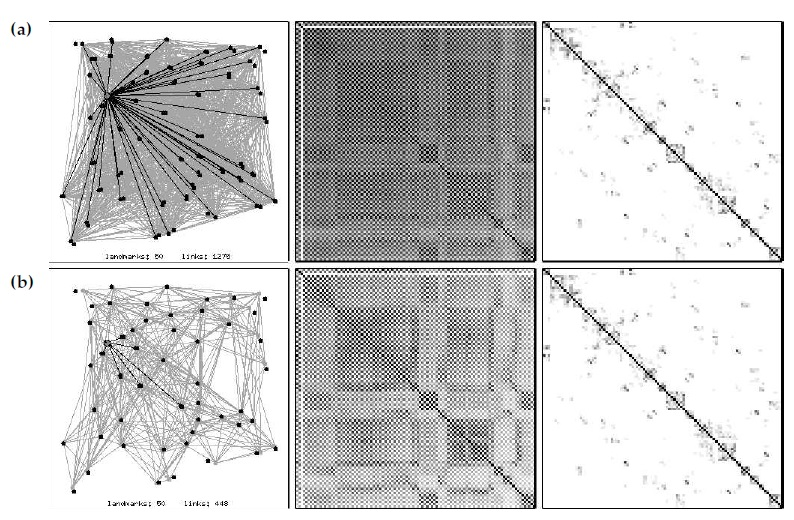
\includegraphics[width=1\linewidth]{126orig}}
	\caption{ ( Рис. 12.6 Сравнение SEIF без разрежения (a) и SEIF с разрежением (b) по 4 активным ориентирам. Сравнение выполнено в имитационной среде с 50 ориентирами. В каждом ряду слева показан набор связей в фильтре, в центре – матрица корреляции, а справа – нормализованная информационная матрица. Очевидно, разреженный SEIF сохраняет намного меньше связей, но результат имеет значительно меньшую степень определённости, что видно по менее выраженной матрице корреляции.) }
	\label{fig:126orig}
\end{figure}

\textbf{12.7	Насколько разреженными должны быть SEIF?}\\

Ключевым вопросом является степень разрежённости, которую следует поддерживать в  SEIF. В частности, степень разрежённости определяет количество активных признаков в SEIF. Разрежённость является компромиссом двух факторов: вычислительной эффективности SEIF и точности результата. При практической реализации алгоритма SEIF рекомендуется найти подходящий компромисс.

«Золотым стандартом» SEIF является EKF, в котором нет разрежения и который не полагается на методы релаксации для восстановления оценок состояния. В следующем сравнении характеризуются три ключевых показателя производительности, которые отделяют разреженные SEIF от EKF. Сравнение основано на имитационной среде робота, в которой робот воспринимает расстояние, направление, и идентификаторы близлежащих ориентиров.

\begin{figure}[H]
	\center{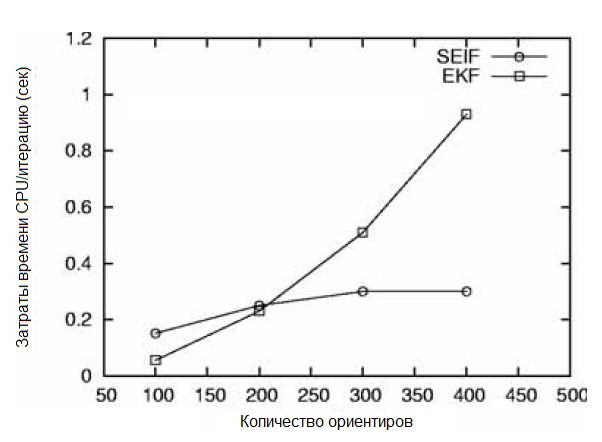
\includegraphics[width=0.7\linewidth]{127orig}}
	\caption{ ( Рис. 12.7    Сравнение  средних затрат процессорного времени для SEIF и EKF.) }
	\label{fig:127orig}
\end{figure}

\begin{figure}[H]
	\center{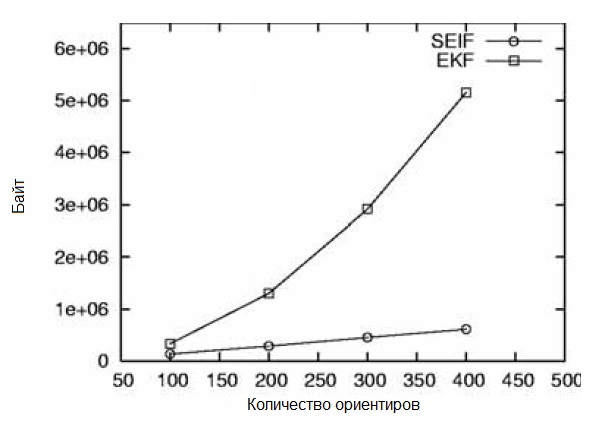
\includegraphics[width=0.7\linewidth]{128orig}}
	\caption{ ( Рис. 12.8    Сравнение среднего использования памяти между SEIF и EKF.) }
	\label{fig:128orig}
\end{figure}

\begin{figure}[H]
	\center{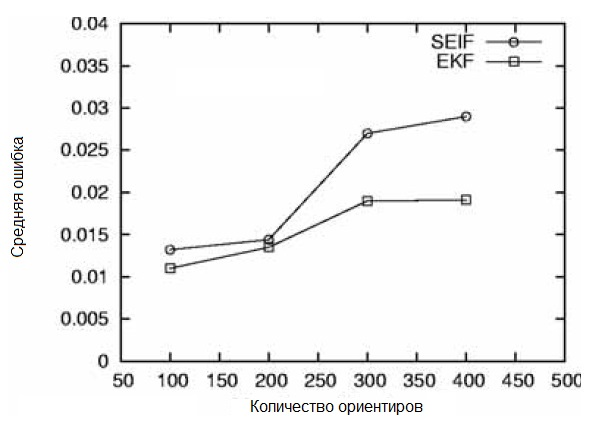
\includegraphics[width=0.7\linewidth]{129orig}}
	\caption{ ( Рис. 12.9 Сравнение квадратного корня среднеквадратичной ошибки между SEIF и EKF.) }
	\label{fig:129orig}
\end{figure}

1.	\textbf{Вычисление.} На Рис. 12.7 показаны вычислительные затраты на обновление SEIF по сравнению с EKF. В обоих случаях реализация оптимизирована. На графике показано основное отличие вероятностного представления в фильтре от информационного. Хотя EKF действительно требуют времени, квадратично зависящего от размера карты, SEIF выполняет выравнивание, что требуют постоянного времени.\\

2.	\textbf{Память.} На Рис. 12.8 приводится сравнение использования памяти EKF и SEIF. И снова, EKF квадратично возрастает, а SEIF возрастёт линейно, в силу разрежённости информационного представления.\\

3.\textbf{	Точность.} Здесь EKF превосходит SEIF потому, что SEIFS требует аппроксимации для поддержания разреженности, а также при восстановлении оценки состояния $\mu_t$. Это показано на Рис. 12.9, где приведены графики ошибки обоих методов в зависимости от размера карты.\\

Один из способов оценки эффекта разреженности – это имитационный эксперимент. На Рис. 12.10 показаны время обновления и ошибка аппроксимации как функция количества активных ориентиров в обновлении SEIF для карты, состоящей из 50 ориентиров. Время обновления монотонно убывает с увеличением количества ориентиров. На Рис. 12.11 показан соответствующий график ошибки, в сравнении EKF с SEIF с различной степенью разреженностью. Сплошной линией показан алгоритм SEIF, а пунктирная соответствует SEIF с явным восстановлением $\mu_t$. Как показано на графике, для 6 активных признаках результаты сходные, при значительной более высокой вычислительной эффективности по сравнению с EKF. Для меньшего количества активных признаков ошибка драматически возрастает. Тщательная реализация SEIF потребует от экспериментатора настройки этого важного параметра, и отображения эффекта влияния на ключевые показатели, как показано на графике. 

\begin{figure}[H]
	\center{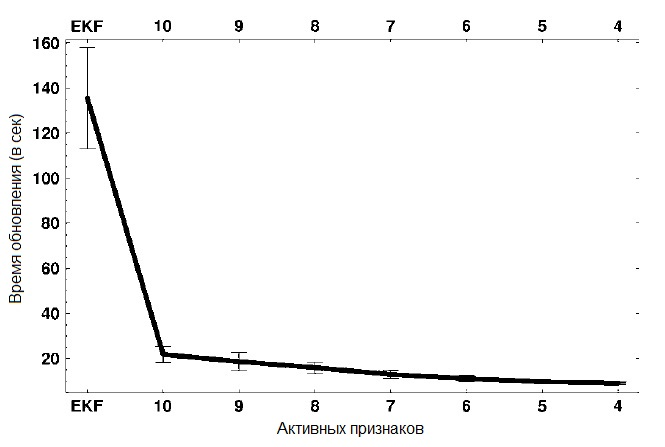
\includegraphics[width=0.7\linewidth]{1210orig}}
	\caption{ ( Рис. 12.10  Время обновления EKF (самая левая точка) и SEIF для различных степеней разреженности на основании количества активных признаков.) }
	\label{fig:1210orig}
\end{figure}

\begin{figure}[H]
	\center{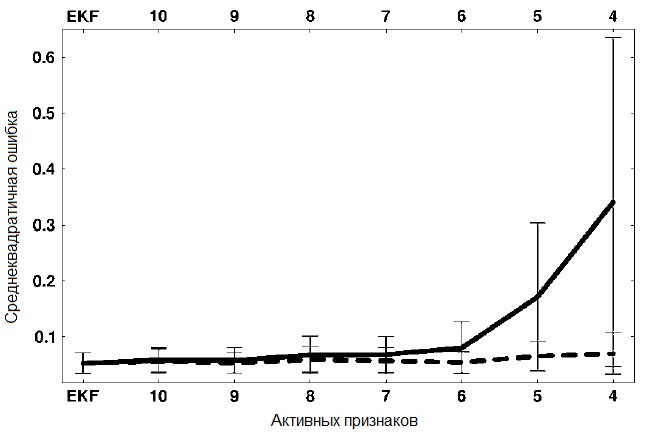
\includegraphics[width=0.7\linewidth]{1211orig}}
	\caption{ ( Рис. 12.11 Ошибка аппроксимации EKF (слева) и SEIF для разных степеней разреженности. На обеих схемах карта состоит из 50 ориентиров.) }
	\label{fig:1211orig}
\end{figure}

\textbf{12.8	Инкрементная ассоциация данных}

Обратим внимание на проблему ассоциации данных в SEIF. Первым методом будет уже знаковый инкрементный подход, жадно идентифицирующий наиболее вероятное соответствие, а затем принимающем это значение как истину. Мы уже встречали экземпляр такого жадного метода ассоциации данных в разделе 10.3 при обсуждении ассоциации данных в EKF. Фактически, единственная разница между жадной инкрементной ассоциацией данных в SEIF и EKF лежит в способе вычисления вероятности ассоциации данных. В общем, вычисление вероятности более сложно в информационном фильтре, чем в вероятностном фильтре, таком как EKF, поскольку информационный фильтр не отслеживает ковариаций.\\

\textbf{12.8.1	Вычисление инкрементных вероятностей ассоциации данных}\\

Как и прежде, вектор ассоциации данных в момент времени $t$ будет обозначаться $c_t$. Жадный инкрементный метод сохраняет набор гипотез ассоциации данных, обозначенных $\hat{c}_{1:t}$. В инкрементном режиме заданы оценки соответствия $\hat{c}_{1:t-1}$ из предыдущих обновлений при вычислении $\hat{c}_t$.  Шаг ассоциации данных затем переходит в оценку наиболее вероятного значения для переменной ассоциации данных $\hat{c}_t$ в момент времени $t$.   Это достигается следующей функцией оценки максимального правдоподобия:\\

(12.41)
\begin{equation*}
\begin{split}
\hat{c}_t&=\underset{c_t}{\text{argmax}}\,\,p(z_t|z_{1:t-1},u_{1:t},\hat{c}_{1:t-1},c_t)\\
&=\underset{c_t}{\text{argmax}}\int p(z_t|y_t,c_t)\underbrace{p(y_t|z_{1:t-1},u_{1:t},\hat{c}_{1:t-1})}_{\bar{\varOmega}_t,\bar{\xi}_t}dy_t\\
&=\underset{c_t}{\text{argmax}}\int\int p(z_t|x_t,y_{c_t},c_t)p(x_t,y_{c_t}|z_{1:t-1},u_{1:t},\hat{c}_{1:t-1})dx_t\,dy_{c_t}
\end{split}
\end{equation*}

Наша запись $p(z_t | x_t, y_{c_t}, c_t)$ модели датчика явно указывает переменную соответствия $c_t$. Явное вычисление этой вероятности за постоянное время невозможно, поскольку включает приведение к пределу почти всех переменных на карте. Однако, тот же самый тип аппроксимации, который был важен для эффективного разрежения, можно применить и здесь.

\begin{figure}[H]
	\center{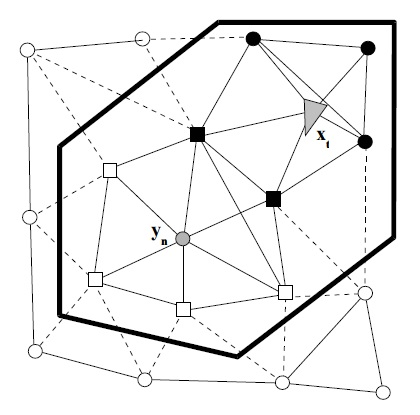
\includegraphics[width=0.6\linewidth]{1212orig}}
	\caption{ ( Рис. 12.12 Комбинированное марковское одеяло признака $y_n$ и наблюдаемых признаков обычно достаточно для аппроксимации апостериорной вероятности местоположения признака, отбрасывая все остальные признаки.) }
	\label{fig:1212orig}
\end{figure}

В частности, обозначим как $m_{c_t}^+$ комбинированное марковское одеяло положения робота $x_t$  и ориентира $y_{c_t}$.   Марковское одеяло – это набор всех признаков на карте, соединённых с роботом или ориентиром $y_{c_t}$. На Рис. 12.12 показан такой набор. Стоит заметить, что $m_{c_t}^+$,  по определению, включает все активные ориентиры.  Разрежённость $\bar{\varOmega}_t$ гарантирует, что $m_{c_t}^+$ содержит только фиксированное количество признаков, независимо от размера карты $N$. Если марковские одеяла $x_t$ и $y_{c_t}$ не пересекаются, добавляются больше признаков, отражающих кратчайший путь в информационном графе между $x_t$ и $y_{c_t}$.

Все оставшиеся признаки будут совместно относиться к $m_{c_t}^-$:\\

(12.42)
$$m_{c_t}^-=m-m_{c_t}^+-\{y_{c_t}\}$$

Множество $m_{c_t}^-$ содержит только признаки с малой степенью воздействия на целевые переменные $x_t$ и $y_{c_t}$.  SEIF аппроксимирует вероятность $p(x_t, y_{c_t}|z_{1:t-1}, u_{1:t}, \hat{c}_{1:t-1})$ в выражении (12.41), игнорируя это непрямое влияние:\\

(12.43)
\begin{equation*}
\begin{split}
p(&x_t, y_{c_t}|z_{1:t-1}, u_{1:t}, \hat{c}_{1:t-1})\\
&=\iint p(x_t, y_{c_t},m_{c_t}^+,m_{c_t}^-|z_{1:t-1}, u_{1:t}, \hat{c}_{1:t-1})dm_{c_t}^+\,dm_{c_t}^-\\
&=\iint p(x_t, y_{c_t}|m_{c_t}^+,m_{c_t}^-,z_{1:t-1}, u_{1:t}, \hat{c}_{1:t-1})\\
&\hspace{10mm} p(m_{c_t}^+|m_{c_t}^-,z_{1:t-1}, u_{1:t}, \hat{c}_{1:t-1})p(m_{c_t}^-|z_{1:t-1}, u_{1:t}, \hat{c}_{1:t-1})dm_{c_t}^+\,dm_{c_t}^-\\
&\approx\int p(x_t, y_{c_t}|m_{c_t}^+,m_{c_t}^-=\mu_{c_t}^-,z_{1:t-1}, u_{1:t}, \hat{c}_{1:t-1})\\
&\hspace{10mm}p(m_{c_t}^+|m_{c_t}^-=\mu_{c_t}^-,z_{1:t-1}, u_{1:t}, \hat{c}_{1:t-1})dm_{c_t}^+
\end{split}
\end{equation*}

Эту вероятность можно вычислить за постоянное время, если набор переменных, задействованных в этом вычислении, не зависит от размера карты (обычно, зависит). Полностью аналогично различным приведённым выше выводам, заметим, что аппроксимация апостериорной вероятности получается простым извлечением субматрицы, соответствующей двум целевым переменным:\\

(12.44)
$$\varSigma_{t:c_t}=F_{x_t,y_{c_t}}^T(F_{x_t,y_{c_t},m_{c_t}^+}^T\varOmega_tF_{x_t,y_{c_t},m_{c_t}^+})^{-1}F_{x_t,y_{c_t}}$$
	
(12.45)
$$\mu_{t:c_t}=\mu_tF_{x_t,y_{c_t}}$$

Это вычисление занимает постоянное время, поскольку включает матрицу размера, независимого от $N$. Из этой гауссовой функции легко можно получить искомую вероятность измерения в Уравнении (12.41).

Так же как в алгоритме EKF SLAM, признаки помечаются новыми, когда правдоподобие  $p(z_t|z_{1:t-1}, u_{1:t}, \hat{c}_{1:t-1}, c_t)$  остаётся ниже порога  $\alpha$. После этого просто установим $\hat{c}_t=N_{t-1}+1$ и $N_t=n_{t-1}+1$, поскольку, в противном случае, размер карты останется неизменным в силу $N_t=N_{t-1}$. Значение $\hat{c}_t$ выбирается таким образом, чтобы максимизировать вероятность ассоциации данных.

Последним препятствием является тот факт, что, иногда, комбинации марковских одеял оказывается недостаточно, поскольку в них нет пути между положением робота и ориентиром, который проверяется на соответствие. Обычно это происходит при замыкании большого цикла в среде. Здесь необходимо дополнить набор признаков $m_{c_t}^+$ набором ориентиров вдоль, по крайней мере, одной траектории между $m_{c_t}$ и положением робота $x_t$. В зависимости от размера цикла количество ориентиров, требуемых для результирующего множества, может зависеть от размера карты $N$. Оставим детальное рассмотрение такого дополнения в качестве упражнения.\\

\textbf{12.8.2	Практические соображения}\\

В общем, инкрементный метод жадной ассоциации данных неустойчив, как обсуждалось в главах, посвящённых EKF SLAM. Ошибочные измерения могут легко привести  к возникновению неверных ассоциаций и вызвать существенные ошибки в оценке SLAM. Стандартным способом избежать этого (как для EKF, так и для SEIF) является создание временного списка ориентиров. Этот метод уже детально обсуждался в подразделе 10.3.3 в контексте EKF SLAM. Во временный список кандидатов, который сохраняется отдельно от SEIF, добавляется любой новый признак, который перед этим не наблюдался. 
\begin{figure}[H]
	\center{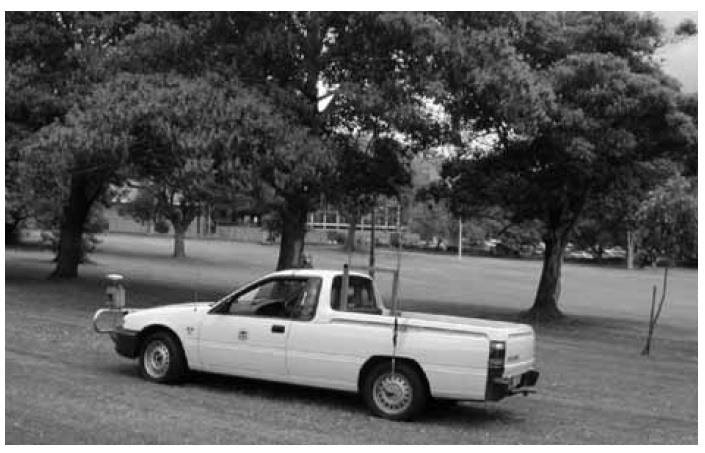
\includegraphics[width=0.6\linewidth]{1213orig}}
	\caption{ ( Рис. 12.13 Автомобиль, используемый в экспериментах, оборудован двухмерным лазерным дальномером и дифференциальной системой GPS. Собственное движение автомобиля измеряется датчиком линейного дифференциального преобразования для угла поворота колес, и энкодером измерения скорости на колесе. На заднем плане видна территория парка Виктория, используемая как среда для тестирования. Изображение принадлежит Хосе Гюванту и Эдуардо Неботу из Австралийского центра полевой робототехники (José Guivant and Eduardo Nebot, Australian Centre for Field Robotics).) }
	\label{fig:1213orig}
\end{figure}
На последующем этапе измерений вновь найденные кандидаты проверяются по всем кандидатам из списка ожидания, совпадения увеличивает вес соответствующих кандидатов, отсутствие наблюдения близлежащего признака уменьшало его вес. Когда вес кандидата превышает определённый порог, он пополняет сеть признаков SEIF.

Заметим, что ассоциация данных нарушает свойство постоянных затрат времени в SEIF. Это происходит при вычислении ассоциации данных, когда необходимо проверить множество признаков. Если бы удалось гарантировать, что все полезные признаки уже присоединены к SEIF короткой траекторией к множеству активных переменных, станет возможным выполнять ассоциацию данных за постоянное время. Таким образом, структура SEIF естественно обеспечивает поиск наиболее вероятного признака, заданного измерением. Однако, такое решение непригодно при закрытии цикла в первый раз, когда верная ассоциация может оказаться слишком далеко в графе соседства SEIF.

Кратко обратим внимание на реализацию SEIF алгоритма на физическом транспортном средстве. Используемые здесь данные являются общим ориентиром в области SLAM. Этот набор данных был собран с помощью оснащённого датчиками автомобилем, который проехал через парк в Сиднее, Австралия.

Автомобиль и окружающая среда показаны на Рис. 12.13 и 12.14, соответственно. Автомобиль оборудован лазерным датчиком расстояния SICK и системой измерения угла поворота руля и поступательной скорости. Лазер предназначался для обнаружения деревьев в окружающей среде, но также обнаружил сотни несуществующих признаков, такие, как углы движущихся по соседней автостраде машин. Данные исходной одометрии, используемые нами, очень некачественные и дают ошибку в несколько сотен метров при использовании интегрирования вдоль пути автомобиля длиной 3,5 км что показано на Рис. 12.14. Плохое качество данных одометрии вкупе с наличием множества ошибочных признаков делает этот набор данных очень подходящим для тестирования алгоритмов SLAM. 

\begin{figure}[H]
	\center{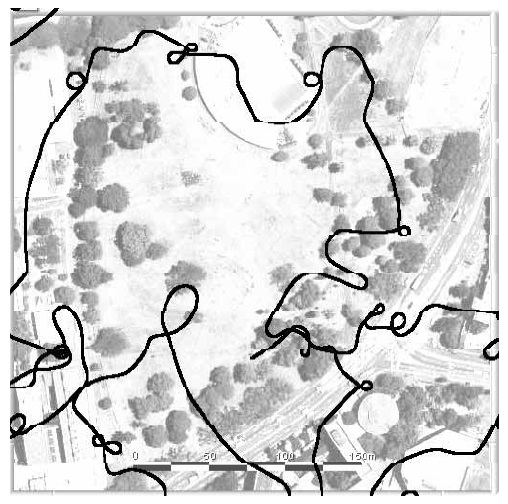
\includegraphics[width=0.6\linewidth]{1214orig}}
	\caption{ (  Рис. 12.14 Тестовая окружающая среда: Участок размером 350 на 350 метров в парке Виктория в Сиднее. Сверху наложен пройденный путь на основе показаний одометрии. Данные и снимок с воздуха принадлежат Хосе Гюванту и Эдуардо Неботу из Австралийского центра полевой робототехники (José Guivant and Eduardo Nebot, Australian Centre for Field Robotics). Результаты принадлежат Майклу Монтемерло из университета Стэнфорда (Michael Montemerlo, Stanford University).) }
	\label{fig:1214orig}
\end{figure}

\begin{figure}[H]
	\center{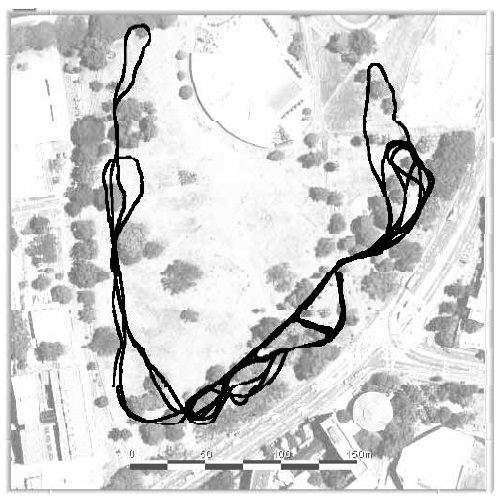
\includegraphics[width=0.6\linewidth]{1215orig}}
	\caption{ ( Рис. 12.15 Траектория пути, восстановленная с помощью SEIF с точностью $\pm1$ м. Собственность Майкла Монтемерло из университета Стэнфорда (Michael Montemerlo, Stanford University)) }
	\label{fig:1215orig}
\end{figure}

\begin{figure}[H]
	\center{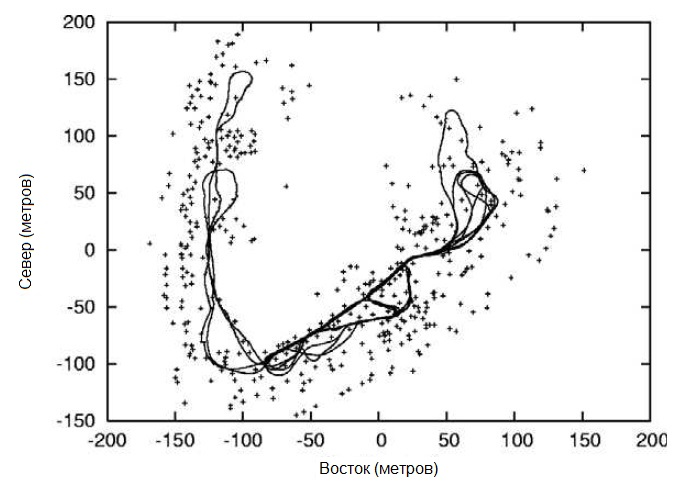
\includegraphics[width=0.8\linewidth]{1216orig}}
	\caption{ ( Рис. 12.16 Наложение оценок местоположений ориентиров и пути автомобиля. Изображения принадлежат Майклу Монтемерло из университета Стэнфорда (Michael Montemerlo, Stanford University)) }
	\label{fig:1216orig}
\end{figure}

Траектория, восстановленная с помощью SEIF, показана на Рис. 12.15. Эта траектория пути вычислительно неотличима от созданного EKF. Средняя ошибка местоположения, измеренная дифференциальным датчиком GPS, составляет менее 0,5 метра, что весьма мало по сравнении с общей длиной пути 3,5 км. Соответствующая карта ориентиров показана на Рис 12.16. Она тоже имеет точность, сравнимую с результатами наиболее современных алгоритмов EKF. В сравнении с алгоритмом EKF  SEIF выполняется, примерно в два раза быстрее и потребляет около четверти памяти, требуемой для EKF. Эта экономия относительно мала, что является результатом малого размера карты. Фактически, наибольшее количество времени было потрачено на предобработку данных датчиков и для карт большего размера относительная экономия будет выше.\\

\textbf{12.9	Ассоциация данных методом ветвей и границ}\\

SEIF позволяет определить полностью иной метод ассоциации данных, который даст оптимальные результаты (хотя, возможно, за экспоненциальное время). Метод построен на трёх ключевых принципах:\\

МЯГКИЕ ОГРАНИЧЕНИЯ АССОЦИАЦИИ ДАННЫХ\\

•	Так же как GraphSLAM, SEIF позволяет добавлять мягкие ограничения ассоциации данных. Для двух заданных признаков $m_i$ и $m_j$, мягкое ограничение ассоциации данных – это всего лишь информационная связь, которая принудительно уменьшает расстояние между $m_i$ и $m_j$. Примеры таких мягких связей уже приводились в предыдущей главе. В разреженных обобщённых информационных фильтрах добавление такой связи представляет собой просто добавление значений в информационную матрицу.\\

•	Мягкие ограничения ассоциации легко удалить. Также, как добавление нового ограничение представляет собой всего лишь локальное добавление в информационную матрицу, удаление представляет собой локальное вычитание. Такая «обратная» операция может быть применена к произвольным связям ассоциации данных, независимо от того, когда они были добавлены, или когда в последний раз наблюдался соответствующий признак. Это делает возможным пересмотр прошлых решений об ассоциации данных.\\

•	Возможность свободно добавлять и удалять ассоциации данных позволяет выполнять поиск по дереву возможных ассоциаций данных  эффективным и целостным способом, как это будет показано ниже.\\

Для разработки алгоритма ассоциации данных методом ветвей и границ, будет полезно определить дерево ассоциации данных, определяющее последовательность решений по ассоциации данных со временем. В каждый момент времени каждый наблюдаемый признак может быть ассоциирован с несколькими другими признаками или же считаться новым, прежде ненаблюдаемым признаком. Результирующее дерево решений об ассоциации данных, от начального момента в момент времени $t=1$ до текущего момента, показано на Рис. 12.17a.  Конечно, дерево экспоненциально разрастётся со временем, поэтому тщательный поиск в нем невозможен. Инкрементный жадный алгоритм, описанный в предыдущем разделе, напротив, следует по единственному пути вдоль дерева, определённому наиболее вероятными ассоциациями данных. Такой путь показан на Рис. 12.17a жирной серой кривой.

Очевидно, если инкрементный жадный метод будет успешно работать, результирующий путь оптимален. Однако, этот метод может и не работать, поскольку в случае неверного решения инкрементынй метод неспособен восстановиться. Более того, неверные решения ассоциации данных вносят ошибки в карту, которые, затем, могут привести к ещё большим ошибкам ассоциации данных. \\

\textbf{12.9.1	Рекурсивный поиск}\\

Этот метод будет обсуждаться в оставшейся части главы и призван обобщить инкрементый жадный алгоритм до полномасштабного алгоритма поиска в оптимальном дереве. Конечно, поиск всех ветвей в дереве выполнять неразумно.\\ 

ПЕРИМЕТР\\

Однако, если сохранять логарифм правдоподобия для всех узлов по \textit{периметру} разрастающегося дерева, оптимальность можно гарантировать. Эта идея показана на Рис. 12.17b: алгоритм SEIF методом ветвей и границ сохраняет не только один путь по дереву ассоциации данных, но весь периметр. Каждый раз при расширении узла (например, с помощью инкрементного максимума правдоподобия),  также оцениваются все альтернативные решения и сохраняются все значения соответствующих правдоподобий.  Это показано на Рис. 12.17b, где приводится логарифм правдоподобия для всего периметра дерева.

Нахождение максимума в Выражении (12.41) предполагает, что логарифм правдоподобия избранного листа выше или равен другому листу на такой же глубине. Поскольку логарифм правдоподобия равномерно убывает с глубиной дерева, можно гарантировать, что ассоциация данных оптимальна, если логарифм правдоподобия избранного листа выше или равен логарифму правдоподобия любого другого узла на периметре. Другими словами, когда узел на периметре получает правдоподобие выше, чем у выбранного листа, это может означать возможность ещё больше увеличить правдоподобие данных, пересмотрев прошлые решения ассоциации данных. В нашем методе такие узлы периметра просто расширяются. Если расширение достигло листа и его значение выше, чем у текущего наилучшего листа, этот лист выбирается для новой ассоциации данных. Поиск прерывается, если все листы периметра имеют меньших или одинаковый параметр правдоподобия с текущим выбранным листом. Этот метод гарантирует сохранение лучшего множества значений переменных для ассоциации данных, но, время от времени, может требовать довольно долгого поиска.\\

\textbf{12.9.2	Вычисление вероятности произвольной ассоциации данных}\\

Для проверки необходимости связи между двумя признаками на карте нам понадобится метод вычисления вероятность их равенства. Этот метод проверки аналогичен методу проверки соответствия в GraphSLAM  в Таблице 11.8 на странице 364 ???. Однако, в SEIF эта проверка приблизительна, поскольку точное вычисление логарифма правдоподобия может потребовать дополнительных вычислений.

\begin{figure}[H]
	\center{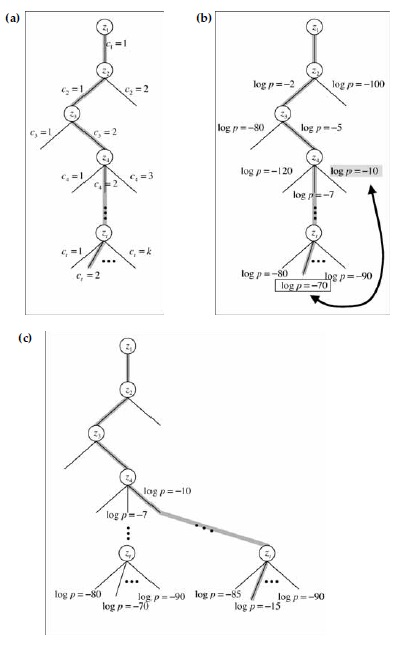
\includegraphics[width=0.8\linewidth]{1217orig}}
	\caption{ ( Рис. 12.17   Дерево ассоциации данных,  коэффициент ветвления которого растёт с увеличением числа ориентиров на карте(a). Алгоритм SEIF на основе дерева поддерживает логарифм правдоподобия для всего периметра расширенных узлов, позволяя находить альтернативные пути(b).  Улучшенная траектория пути (c). ) }
	\label{fig:1217orig}
\end{figure}

\begin{table}[H]
\begin{center}
\begin{tabular}{|l|}
\hline
{}\\
1:\textbf{ Algorithm SEIF\_correspondence\_test}$(\varOmega,\mu,m_j,m_k):$ \\
2:\hspace{5mm}$\textit{пусть }\,B(j)\,\textit{будет одеялом }\,m_j$\\
3:\hspace{5mm}$\textit{пусть }\,B(k)\,\textit{будет одеялом }\,m_k$\\
4:\hspace{5mm}$B=B(j)\cup B(k)$\\
5:\hspace{5mm}$\textit{if}\,B(j)\cap B(k)=\emptyset$\\
6:\hspace{10mm}$\textit{добавить признаки по кратчайшему пути между }\,m_i\,\textit{и}\,m_j\,\textit{и }\,B$\\
7:\hspace{5mm}$\textit{endif}$\\
8:\hspace{5mm}$F_B=\left(\begin{array}{ccccccccccc}
0...0&1&0&0&0...0&{}&\cdots&{}&{}&{}&{}\\
0...0&0&1&0&0...0&{}&\cdots&{}&{}&{}&{}\\
0...0&0&0&1&0...0&{}&\cdots&{}&{}&{}&{}\\
{}&\cdots&{}&{}&0...0&1&0&0&0...0&{}&{}\\
{}&\cdots&{}&{}&0...0&0&1&0&0...0&{}&{}\\
{}&\cdots&{}&{}&0...0&0&0&1&0...0&{}&{}\\
{}&{}&{}&{}&{}&{}&{}&{}&{}&\ddots&{}\\
{}&{}&{}&{}&\cdots&{}&{}&{}&{}&{}&0...0\\
{}&{}&{}&{}&\cdots&{}&{}&{}&{}&{}&0...0\\
\end{array} \right)$\\
9:\hspace{25mm}$(\textit{размер}\,(3N+3)\,\textit{на}\,3|B|)$\\
10:\hspace{4mm}$\varSigma_B=(F_B\varOmega F_B^T)^{-1}$\\
11:\hspace{4mm}$\mu_B=\varSigma_BF_B\xi$\\
12:\hspace{4mm}$F_\varDelta=\left(\begin{array}{ccccc}0...0&1\quad0&0...0&-1\quad0&0...0\\
0...0&\underbrace{0\quad1}_{\text{признак}\,m_j}&0...0&\underbrace{0\quad-1}_{\text{признак}\,m_j}&0...0\\
\end{array}\right)$\\
13:\hspace{4mm}$\varSigma_\varDelta=(F_\varDelta\varOmega F_\varDelta^T)^{-1}$\\
14:\hspace{4mm}$\mu_\varDelta=\varSigma_\varDelta F_\varDelta\xi$\\
15:\hspace{4mm}$\textit{return}\,\det(2\pi\varSigma_\varDelta)^{-\frac{1}{2}}\exp\{-\frac{1}{2}\mu_\varDelta^T\varSigma_\varDelta^{-1}\mu_\varDelta\}$\\
{}\\
\hline
\end{tabular}
\caption{(Таблица 12.6  Проверка соответствия для SEIF SLAM.)}
\end{center}
\end{table}

В Таблице 12.6 приведён алгоритм, который проверяет вероятность того, что два признака на карте соответствуют одному ориентиру. Такой проверки достаточно для реализации метода жадной ассоциации данных. Ключевое вычисление здесь состоит в восстановлении объединённой ковариации и среднего вектора на небольшом множестве признаков карты $B$. Для определения идентичности двух признаков на карте, в SEIF необходимо учитывать информационные связи между ними. Технически, чем больше связей принимается во внимание, тем более точным будет результат, но лишь ценой дополнительных вычислений. 
На практике обычно достаточно идентифицировать два \textit{марковских одеяла} интересующих признаков. \\

МАРКОВСКОЕ ОДЕЯЛО\\
Марковское одеяло для признака - это сам признак и все прочие признаки, соединённые с ним ненулевым элементом информационной матрице. В большинстве случаем марковские одеяла пересекаются. Если этого не происходит, алгоритм в Таблице 12.6 находит путь между ориентирами (который должен существовать, если оба признака наблюдались одним и тем же роботом).

Затем алгоритм в Таблице 12.6 вырезает локальные информационную матрицу и информационный вектор, выполняя тот же самый математический «фокус», который позволял эффективный осуществлять разрежение: SEIF выбрасывает признаки за пределами марковских одеял. В результате, в алгоритме SEIF появляется эффективный метод вычисления искомой вероятности, пусть и приблизительный (из-за отбрасывания переменных), но очень хорошо работающий на практике.

Результат интересен тем, что не только позволяет SEIF принимать решения по ассоциации данных, но и предоставляет способ вычисления логарифма правдоподобия такого решения. Логарифм результата такой процедуры соответствует логарифму правдоподобия отдельного элемента данных, а суммирование по траектории в дереве ассоциации данных даёт логарифм правдоподобия всех данных для конкретной ассоциации.

\textbf{12.9.3	Ограничения эквивалентности}\\

Как только два признака на карте были определены в качестве эквивалентных при поиске ассоциации данных, в SEIF добавляется мягкая связь в информационную матрицу. Допустим, первый признак $m_i$, а второй - $m_j$. Мягкая связь ограничивает их местоположение одним и тем же местом с помощью следующего экспоненциально-квадратичного ограничения\\

(12.46)
$$\exp\{-\frac{1}{2}(m_i-m_j)^T\,C(m_i-m_j)\}$$

Здесь $C$ - диагональная матрица штрафа типа\\

(12.47)
$$C=\left(\begin{array}{ccc}
\infty&0&0\\
0&\infty&0\\
0&0&\infty\\
\end{array}\right)$$

На практике диагональные элементы $C$ большими положительными значениями, и чем больше эти значения, тем сильнее ограничение.

Легко увидеть, что ненормализованный гауссиан (12.46) может быть записан в информационной матрице в виде связи между $m_i$ и $m_j$. Определим матрицу проекции\\

(12.48)
$$F_{m_i-m_j}=\left(\begin{array}{ccccc}
0...0&1\quad0\quad0&0...0&-1\quad0\quad0&0...0\\
0...0&0\quad1\quad0&0...0&0\quad-1\quad0&0...0\\
0...0&\underbrace{0\quad0\quad1}_{m_i}&0...0&\underbrace{0\quad0\quad-1}_{m_j}&0...0\\
\end{array}\right)$$

Матрица проецирует состояние $y_t$ в виде разницы $m_i-m_j$. Отсюда, выражение (12.46) становится\\

(12.49)
\begin{equation*}
\begin{split}
\exp&\{-\frac{1}{2}(F_{m_i-m_j}y_t)^T\,C\,(F_{m_i-m_j}y_t)\}\\
&=\exp\{-\frac{1}{2}y_t^T[F_{m_i-m_j}^T\,C\,F_{m_i-m_j}]y_t\}
\end{split}
\end{equation*}

Для реализации этого мягкого ограничения в SEIF необходимо добавить $F_{m_i-m_j}\,C\,F_{m_i-m_j}$ к информационной матрице, оставляя информационный вектор неизменным:\\

(12.50)
$$\varOmega_t\longleftarrow\varOmega_t+F_{m_i-m_j}^TCF_{m_i-m_j}$$

Конечно, добавочный член разрежен, поскольку содержит ненулевые элементы вне главной диагонали только между признаками $m_i$ и $m_j$. После добавления мягкой связи ее можно удалить с помощью инверсии\\

(12.51)
$$\varOmega_t\longleftarrow\varOmega_t-F_{m_i-m_j}^TCF_{m_i-m_j}$$

Это удаление может быть выполнено вне зависимости от времени, которое прошло с момента добавления ограничения в фильтр. Однако, требуется внимательность, чтобы не позволить SEIF удалить несуществующее ограничение, в противном случае информационная матрица уже не будет неотрицательно определённой, и результирующая оценка может не соответствовать правильному вероятностному распределению.\\

\textbf{12.10	Практические соображения}\\

В любой конкурентной реализации этого метода обычно будет существовать только небольшое количество путей ассоциации данных, применимых в произвольный момент времени. При замыкании цикла в среде внутри помещения обычно имеется только три разумные гипотезы: закрытие, продолжить влево и продолжить вправо. Но вероятность быстро уменьшается, поэтому количество проходов поиска по дереву обычно достаточно мало. 

\begin{figure}[H]
	\center{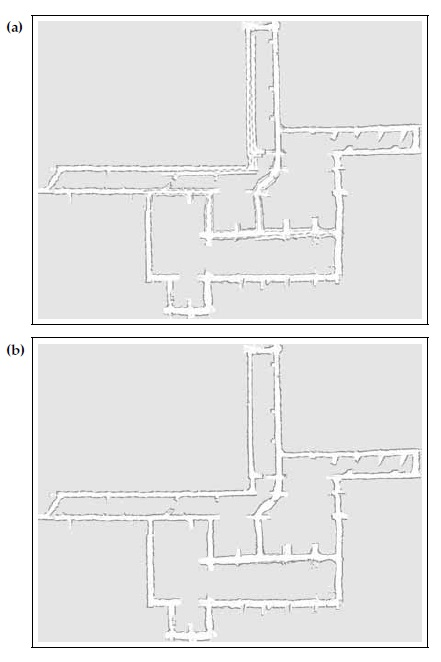
\includegraphics[width=0.8\linewidth]{1218orig}}
	\caption{ ( Рис. 12.18  Карта с инкрементным наложением сканирований по методу ML(a) и полной рекурсивной ассоциации данных по методу ветвей и границ (b). Изображения принадлежат Дирку Хенелу, университет Фрайбурга (Dirk Hähnel, University of Freiburg).) }
	\label{fig:1218orig}
\end{figure}

Одним из способов увеличения эффективности ассоциации данных является учёт отрицательной информации измерения. Датчики расстояния, используемые в предложенных реализациях, возвращают как положительную, так и отрицательную информацию о наличии объектов окружающего мира. Положительная информация – это обнаружения объектов, отрицательная описывает расстояние между датчиком и объектом. Тот факт, что робот не смог обнаружить объект ближе текущих показаний датчика, даёт информацию об отсутствии объекта в диапазоне измерений. 

\begin{figure}[H]
	\center{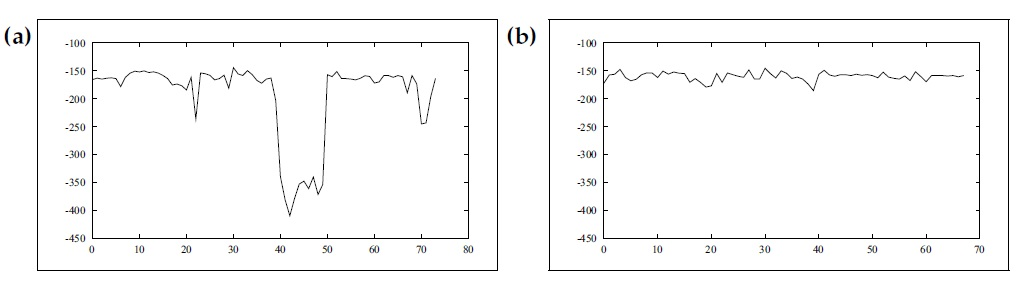
\includegraphics[width=1\linewidth]{1219orig}}
	\caption{ ( Рис. 12.19  Логарифм правдоподобия настоящего измерения как функция времени.  Меньшее правдоподобие вызвано неверной ассоциацией (a). Логарифм правдоподобия при рекурсивном восстановлении с помощью поиска по дереву (b). Успешность определяется по отсутствию выраженных провалов.) }
	\label{fig:1219orig}
\end{figure}

\begin{figure}[H]
	\center{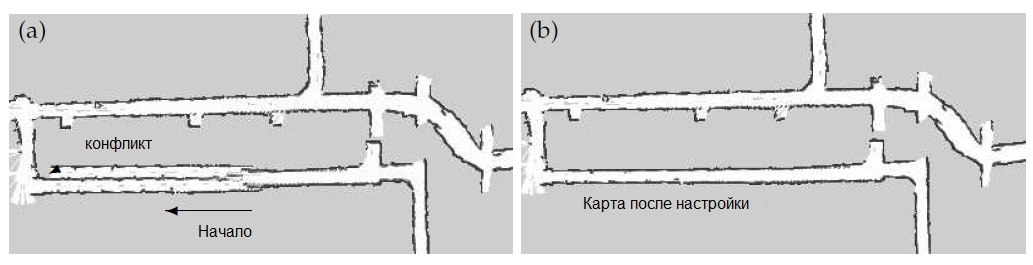
\includegraphics[width=1\linewidth]{1220orig}}
	\caption{ ( Рис. 12.20 Пример метода ассоциации данных на основе деревьев:  при закрытии большого цикла, робот ошибочно принимает решение о наличии второго, параллельного пути (a). Эта модель теряет целостность, когда робот достигает правого поворота. В этой точке выполняется рекурсивный поиск лучшего метода ассоциации данных, что приводит к построению карты справа (b).) }
	\label{fig:1220orig}
\end{figure}

Метод, который оценивает эффект нового ограничения на общее правдоподобие, учитывает оба типа информации - и положительную, и отрицательную. Это выполняется вычислением попарного соответствия (или несоответствия) двух проходов сканирования при оценке положения. При использовании датчиков расстояния одним из способов получения комбинации положительной и отрицательной информации является наложение сканирования на локальную карту сетки занятости, построенную по результатам другого сканирования. Это очевидный способ определить примерную вероятность соответствия двух локальных карт, с учётом положительной, и отрицательной информации.

В оставшейся части этого раздела описаны практические результаты, полученные при использовании SEIF с ассоциацией данных методом деревьев. Слева на Рис. 12.18a показан результат инкрементной ассоциации данных по методу максимального правдоподобия, что эквивалентно регулярному инкрементному сравнению проходов сканирования. Очевидно, некоторые коридоры на карте показаны дважды, показывая недостатки метода максимального правдоподобия. Для сравнения справа показан результат.  Хорошо видно, что карта более точная, по сравнению с созданной методом инкрементного максимального правдоподобия.

\begin{figure}[H]
	\center{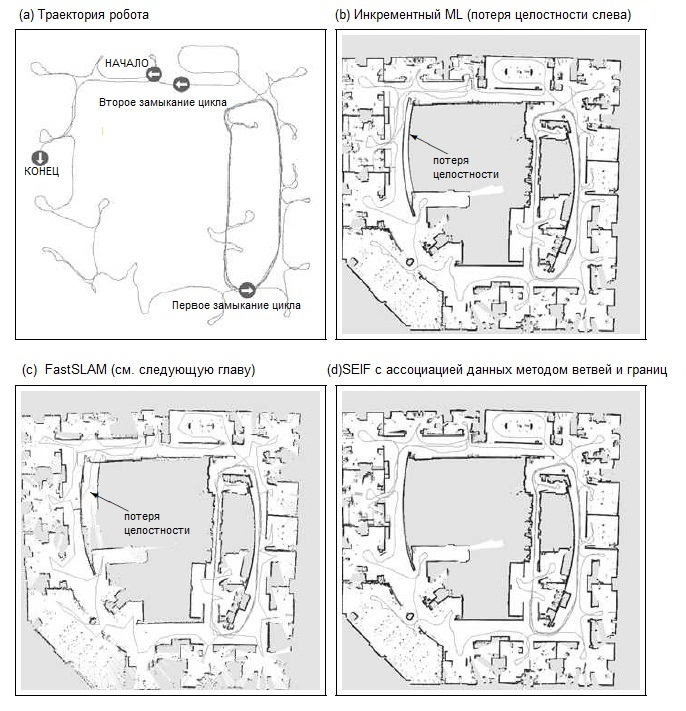
\includegraphics[width=1\linewidth]{1221orig}}
	\caption{ ( Рис. 12.21 Траектория робота (a). Инкрементный ML (сравнение сканирований)(b),  Fast SLAM(c). SEIF с ленивой ассоциацией данных (d). Изображение принадлежит Дирку Хенелу, университет Фрайбурга (Dirk Hähnel, Univer- sity of Freiburg).) }
	\label{fig:1221orig}
\end{figure}

На Рис. 12.19a показан логарифм правдоподобия самого последнего измерения (не всей траектории), который существенно падает с потерей целостности карты. В этой точке SEIF выполняет поиск альтернативных значений ассоциации данных. Он быстро обнаруживает «верное», создавая карту, изображённую на Рис. 12.18b. Рассматриваемая зона показана на Рис. 12.20, иллюстрирующем 
момент резкого спада логарифма правдоподобия. Сам логарифм правдоподобия измерения показан на Рис. 12.19b.

Наконец, на Рис. 12.21 сравниваются различные методы в контексте картографирования большого здания с несколькими циклами.\\

\textbf{12.11	SLAM с несколькими роботами}\\

Алгоритм SEIF также применим к задачам \textit{SLAM с использованием нескольких роботов}. Задача использования нескольких роботов в SLAM включает независимое исследование и картографирование несколькими роботами с конечной целью интеграции нескольких карт в одну монолитную карту. Во многих отношениях задача SLAM с несколькими роботами напоминает картографирование одним роботом, когда данные необходимо интегрировать в единое апостериорное распределение со временем. Однако, задача для нескольких роботов существенно сложнее в ряде аспектов:\\

•	При отсутствии априорной информации об относительном местоположении двух роботов проблема соответствия становится \textit{глобальной}. Главным образом, любые два признака на карте могут соответствовать, и робот способен определить верные соответствия только путём сравнения многих признаков .\\

•	Все карты будут получены в локальных системах координат, которые могут отличаться по абсолютным местоположениям и ориентациям по направлению. Перед интегрированием двух карт их необходимо совместить путём смещения и поворота. В SEIF это потребует повторной линеаризации информационной матрицы и вектора.\\

•	Степень наложения двух карт заранее неизвестна. Например, роботы могут действовать на разных этажах здания с одинаковой поэтажной планировкой. В такой ситуации возможность различить карты будет основана на мелких отличающихся признаках окружающей среды, например, по-разному расставленная мебель.\\

В этом разделе будут эскизно намечены некоторые идеи реализации алгоритма картографирования с помощью нескольких роботов. Будет представлен алгоритм интегрирования двух карт после установки соответствия. Также будут обсуждаться, без приведения доказательства, методы установки глобального соответствия для SLAM с использованием нескольких роботов.\\

\textbf{12.11.1	Интегрирование карт}

Критические моменты для слияния карт с известным соответствием показаны в Таблице 12.7. Этот алгоритм принимает на вход два локальных апостериорных Распределения, выраженные в информационном виде $\varOmega^j$, $\xi^j$ и $\varOmega^k$, $\xi^k$, соответственно. Также требуются три других элемента\\

1.	Набор значений линейного смещения $d$\\

2.	Относительный  угол поворота $\alpha$\\

3.	Набор соответствия признаков  $\mathcal{C}^{j,k}$

\begin{table}[H]
\begin{center}
\begin{tabular}{|l|}
\hline
{}\\
1:\textbf{ Algorithm SEIF\_map\_fusion}$(\varOmega^j,\xi^j,\varOmega^k,\xi^k,d,\alpha,\mathcal{C}):\qquad$\\
2:\hspace{5mm}$\varDelta=(d_x\,\,d_y\,\,\alpha\,\,d_x\,\,d_y\,\,0\,\,...\,\,d_x\,\,d_y\,\,0)^T$\\
3:\hspace{5mm}$\mathcal{A}=\left(\begin{array}{ccccccc}
\cos\alpha&\sin\alpha&0&{}&{}&\ldots&0\\
-\sin\alpha&\cos\alpha&0&{}&{}&{}&\vdots\\
0&0&1&{}&{}&{}&{}\\
{}&{}&{}&\ddots&{}&{}&{}\\
{}&{}&{}&{}&\cos\alpha&\sin\alpha&0\\
\vdots&{}&{}&{}&-\sin\alpha&\cos\alpha&0\\
0&\ldots&{}&{}&0&0&1\\
\end{array} \right)$\\
4:\hspace{5mm}$\varOmega^{j\longrightarrow k}=\mathcal{A}\varOmega^j\mathcal{A}^T$\\
5:\hspace{5mm}$\xi^{j\longrightarrow k}=\mathcal{A}(\xi^j-\varOmega^{j\longrightarrow k}\varDelta)$\\
6:\hspace{5mm}$\varOmega=\left(\begin{array}{cc}\varOmega^k&0\\
0&\varOmega^{j\longrightarrow k}\\\end{array} \right)$\\
7:\hspace{5mm}$\xi=\left(\begin{array}{c}\xi^k\\
\xi^{j\longrightarrow k}\\\end{array} \right)$\\
8:\hspace{5mm}$\textit{for any pair}\,(m_j,m_k)\in \mathcal{C}^{j,k}\,\textit{do}$\\
9:\hspace{10mm}$F=\left(\begin{array}{ccccc}
0...0&1\quad0\quad0&0...0&-1\quad0\quad0&0...0\\
0...0&0\quad1\quad0&0...0&0\quad-1\quad0&0...0\\
0...0&\underbrace{0\quad0\quad1}_{m_j}&0...0&\underbrace{0\quad0\quad-1}_{m_k}&0...0\\
\end{array}\right)$\\
10:\hspace{9mm}$\varOmega\longleftarrow\varOmega+F^T\left(\begin{array}{ccc}\infty&0&0\\0&\infty&0\\0&0&\infty\\\end{array}\right)\,F$\\
11:\hspace{4mm}$\textit{endfor}$\\
12:\hspace{4mm}$\textit{return}\,\,\varOmega,\xi$\\
{}\\
\hline
\end{tabular}
\caption{(Таблица 12.7    Цикл слияния карт для картографирования алгоритмом SEIF несколькими роботами.)}
\end{center}
\end{table}

Вектор смещения $d = (d_x\,\,d_y)^T$ и поворот $\alpha$ определяет относительную ориентацию карт двух роботов. В частности, $j$-е положение робота $x^j$ и признаки карты $j$-го робота проектируются в систему координат $k$-го робота с помощью поворота на $\alpha$ с последующим параллельным переносом $d$. Здесь будем использовать обозначение “$j\longrightarrow k$” для координат элемента карты $j$-го робота, выраженного в системе координат $k$-го робота.\\

1.	Для положения $j$-го робота $x_t^j$\\

(12.52)
$$\underbrace{\left(\begin{array}{c}x^{j\longrightarrow k}\\y^{j\longrightarrow k}\\\theta^{j\longrightarrow k}\\\end{array}\right)}_{x_t^{j\longrightarrow k}}=\left(\begin{array}{c}d_x\\d_y\\\alpha\\\end{array}\right)+\left(\begin{array}{ccc}\cos\alpha&\sin\alpha&0\\-\sin\alpha&\cos\alpha&0\\0&0&1\\\end{array}\right)\underbrace{\left(\begin{array}{c}x^j\\y^j\\\theta^j\\\end{array}\right)}_{x_t^j}$$

2.	Для каждого признака карты $j$-го робота $m_i^j$\\

(12.53)
$$\underbrace{\left(\begin{array}{c}m^{j\longrightarrow k}_{i,x}\\m^{j\longrightarrow k}_{i,y}\\m^{j\longrightarrow k}_{i,s}\\\end{array}\right)}_{m_t^{j\longrightarrow k}}=\left(\begin{array}{c}d_x\\d_y\\0\\\end{array}\right)+\left(\begin{array}{ccc}\cos\alpha&\sin\alpha&0\\-\sin\alpha&\cos\alpha&0\\0&0&1\\\end{array}\right)\underbrace{\left(\begin{array}{c}m^j_{i,x}\\m^j_{i,y}\\m^j_{i,s}\\\end{array}\right)}_{m_t^j}$$

Эти две проекции выполняются в строках со 2 по 5 алгоритма \textbf{SEIF\_map \_fusion} в Таблице 12.7. На этом этапе выполняются локальный поворот и смещение информационной матрицы и информационного вектора, что сохраняет разрежённость SEIF. После этого выполняется слияние карт путём построения единой апостериорной карты в строках 6 и 7. На финальном шаге алгоритма слияния определяется список соответствия $C^{j,k}$. Это множество состоит из пар признаков $(m_j, m_k)$, которые взаимно соответствуют карте робота $j$ и роботу $k$. Слияние выполняется аналогично мягким ограничениям эквивалентности, упоминаемым в подразделе 12.9.3. Для любых двух соответствующих признаков просто выполняется добавление больших значений элементам информационной матрицы, соединяющим эти признаки.

Заметим, что альтернативным способом выполнить слияние карт будет свернуть соответствующие строки и столбцы результирующей информационной матрицы и вектора. Следующий пример показывает операцию сворачивания признаков 2 и 4 в фильтре, которая может произойти, когда состояния в списке соответствия признаков 2 и 4 идентичны:\\

(12.54)
$$\left(\begin{array}{cccc}\varOmega_{11}&\varOmega_{12}&\varOmega_{13}&\varOmega_{14}\\
\varOmega_{21}&\varOmega_{22}&\varOmega_{23}&\varOmega_{24}\\
\varOmega_{31}&\varOmega_{32}&\varOmega_{33}&\varOmega_{34}\\
\varOmega_{41}&\varOmega_{42}&\varOmega_{43}&\varOmega_{44}\\\end{array}\right)\longrightarrow\left(\begin{array}{ccc}\varOmega_{11}&\varOmega_{12}+\varOmega_{14}&\varOmega_{13}\\\varOmega_{21}+\varOmega_{41}&\varOmega_{22}+\varOmega_{42}+\varOmega_{24}+\varOmega_{44}&\varOmega_{23}+\varOmega_{43}\\\varOmega_{31}&\varOmega_{32}+\varOmega_{34}&\varOmega_{33}\\\end{array}\right)$$

(12.55)
$$\left(\begin{array}{c}\xi_1\\\xi_2\\\xi_3\\\xi_4\\\end{array}\right)\longrightarrow\left(\begin{array}{c}\xi_1\\\xi_2+\xi_4\\\xi_3\\\end{array}\right)$$

Сворачивание использует аддитивность информационного состояния.\\

\textbf{12.11.2	Математический вывод интеграции карт}\\

Для этого вывода будет достаточно заданных информационной матрицы и векторов сдвига, указанных в (12.52) и (12.53). Определим переменные $\delta_x$, $\delta_m$, и $A$ следующим образом:\\

(12.56)
$$\delta_x=(d_x\,\,d_y\,\,\alpha)^T$$

(12.57)
$$\delta_m=(d_x\,\,d_y\,\,0)^T$$

(12.58)
$$A=\left(\begin{array}{ccc}\cos\alpha&\sin\alpha&0\\-\sin\alpha&\cos\alpha&0\\0&0&1\\\end{array}\right)$$

Перепишем (12.52) и (12.53) в виде\\

(12.59)
$$x_t^{j\longrightarrow k}=\delta_x+Ax_t^j$$

(12.60)
$$m_t^{j\longrightarrow k}=\delta_m+Am_i^j$$

Для полного вектора состояний получаем\\

(12.61)
$$y_t^{j\longrightarrow k}=\varDelta+\mathcal{A}y_t^j$$
c

(12.62)
$$\varDelta=(\delta_r\,\,\delta_m\,\,\delta_m\,\,...\,\,\delta_m)^T$$
 
(12.63)
$$\mathcal{A}=\left(\begin{array}{cccc}A_r&0&\cdots&0\\
0&A_m&\cdots&0\\
\vdots&\vdots&\ddots&\vdots\\
0&0&\cdots&A_m\\
\end{array}\right)$$

Требуемое преобразование координат в информационном пространстве выполняется схожим образом. Пусть апостериорная вероятность для $j$-го робота в момент времени $t$ будет определена информационной матрицей $\varOmega^j$ и информационным вектором $\xi^j$ для сдвига и поворота используется следующее преобразование:\\

(12.64)
\begin{equation*}
\begin{split}
p(y^{j\longrightarrow k}&|z_{1:t}^j,u_{1:t}^j)\\
&=\eta\,\exp\{-\frac{1}{2}y^{j\longrightarrow k,T}\varOmega^{j\longrightarrow k}y^{j\longrightarrow k}+y^{j\longrightarrow k,T}\xi^{j\longrightarrow k}\}\\
&=\eta\,\exp\{-\frac{1}{2}(\varDelta+\mathcal{A}y^j)^T\varOmega^{j\longrightarrow k}(\varDelta+\mathcal{A}y^j)+(\varDelta+\mathcal{A}y^j)^T\xi^{j\longrightarrow k}\}\\
&=\eta\,\exp\{ -\frac{1}{2}y^{jT}\mathcal{A}^T\varOmega^{j\longrightarrow k}\mathcal{A}y^j+y^{jT}\varOmega^{j\longrightarrow k}\varDelta-\underbrace{\frac{1}{2}\varDelta^T\varOmega^{j\longrightarrow k}\varDelta}_{\text{const.}}\\
&\hspace{55mm}+\underbrace{\varDelta^T\xi^{j\longrightarrow k}}_{\text{const.}}+y^{jT}\mathcal{A}^T\xi^{j\longrightarrow k}\} \\
&=\eta\,\exp\{-\frac{1}{2}y^{jT}\mathcal{A}^T\varOmega^{j\longrightarrow k}\mathcal{A}y^j+y^{jT}\varOmega^{j\longrightarrow k}\varDelta+y^{jT}\mathcal{A}^T\xi^{j\longrightarrow k}\}\\
&=\eta\,\exp\left\lbrace -\frac{1}{2}y^{jT}\underbrace{\mathcal{A}^T\varOmega^{j\longrightarrow k}\mathcal{A}}_{\varOmega^j}y^j+y^{jT}\underbrace{(\varOmega^{j\longrightarrow k}\varDelta+\mathcal{A}^T\xi^{j\longrightarrow k})}_{\xi^j}\right\rbrace 
\end{split}
\end{equation*}

Таким образом, получается\\

(12.65)
$$\varOmega^j=\mathcal{A}^T\varOmega^{j\longrightarrow k}\mathcal{A}$$

(12.66)
$$\xi^j=(\varOmega^{j\longrightarrow k}\varDelta+\mathcal{A}^T\xi^{j\longrightarrow k})$$

Из $\mathcal{A}^{-1}=\mathcal{A}^T$ следует, что\\

(12.67)
$$\varOmega^{j\longrightarrow k}=\mathcal{A}\varOmega^j\mathcal{A}^T$$

$$\xi^{j\longrightarrow k}=\mathcal{A}(\xi^j-\varOmega^{j\longrightarrow k}\varDelta)$$

Это доказывает правильность участка алгоритма в строках со 2 до 7 в Таблице 12.7. Оставшиеся мягкие ограничения эквивалентности напрямую следуют из обсуждения в подразделе 12.9.3. \\

\textbf{12.11.3	Установка соответствия}\\

Оставшаяся часть задачи относится к установке соответствия между разными картами, и вычисление поворота $\alpha$ и параллельного переноса $\delta$. Существует огромное множество подходящих методов, поэтому алгоритм будет приводиться эскизно. Очевидно, задача состоит в необходимости, потенциально, совмещать большое количество признаков на обеих локальных картах.

Канонический алгоритм для карт на основе признаков может выполнять кэшировние конфигурации достаточно близко расположенных ориентиров таким образом, чтобы локальные конфигурации давали хорошие признаки-кандидаты для соответствия. Например, можно идентифицировать множество $m$ близко расположенных ориентиров (для небольшого числа $m$), и вычислить относительные расстояния и углы между ними. Такой вектор расстояний или углов послужит статистическим показателем, с помощью которого можно выполнить сравнение двух карт. Используя хэш-таблицы или kd-деревья, можно эффективно повысить их доступность, поэтому ответ на вопрос «соответствуют ли следующие m ориентиров для карты $j$-робота каким-либо $m$ ориентирам на карте робота $k$?» можно получить очень легко, по крайней мере, оценочно. После определения начального соответствия можно легко вычислить $d$ и $\alpha$ минимизируя квадрат расстояния между этими $m$ признаками обеих карт.

Слияние выполняется следующим образом: сначала вызывается оператор слияния, используя $d$, $\alpha$ и $C$, вычисленных из $m$ локальных признаков обеих карт. Затем идентифицируются дополнительные ориентиры, для которых проверка соответствия в Таблице 12.6 генерирует вероятность меньше пороговой. Если такие пары ориентиров не найдены, выполнение алгоритма прерывается.

Сравнение обоих компонентов объединённых карт, особенно близко расположенных ориентиров, для которых нет соответствия, даст критерий результирующего сравнения. Формально, слияние карт происходит сразу же после прерывания процесса поиска, если результирующее уменьшение общего правдоподобия в логарифмическом виде сдвинулось согласно количеству свёрнутых признаков с постоянным коэффициентом. Это эффективно реализует байесовскую функцию оценки MAP с экспоненциальным априорным распределением по количеству признаков окружающего пространства.

В общем случае, заметим, что поиск оптимального соответствия NP- сложен, но алгоритмы нахождения экстремума на практике работают чрезвычайно эффективно.\\

\textbf{12.11.4	Пример}\\

На Рис. 12.22 приведён пример из восьми локальных карт. Эти карты получены разбиением эталонного набора данных, обсуждаемого выше, на 8 непересекающихся последовательностей, и выполнением алгоритма SEIF на каждой по отдельности.

\begin{figure}[H]
	\center{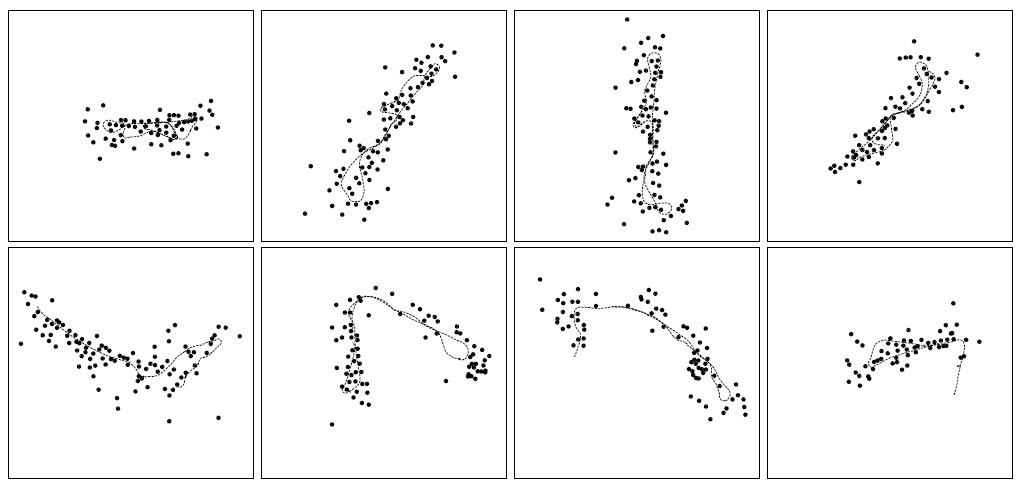
\includegraphics[width=0.8\linewidth]{1222orig}}
	\caption{ ( Рис. 12.22   Восемь локальных карт, полученных разбиением набора данных на восемь последовательностей.) }
	\label{fig:1222orig}
\end{figure}

\begin{figure}[H]
	\center{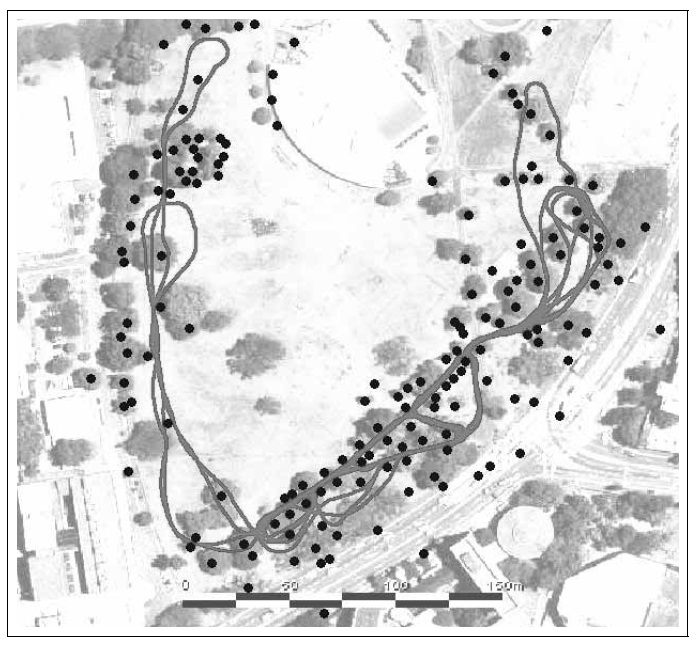
\includegraphics[width=0.8\linewidth]{1223orig}}
	\caption{ ( Рис. 12.23  Результат работы SLAM с помощью нескольких роботов, описанного в этой главе. Изображение принадлежит Юфенг Лю (Yufeng Liu).) }
	\label{fig:1223orig}
\end{figure}

\begin{figure}[H]
	\center{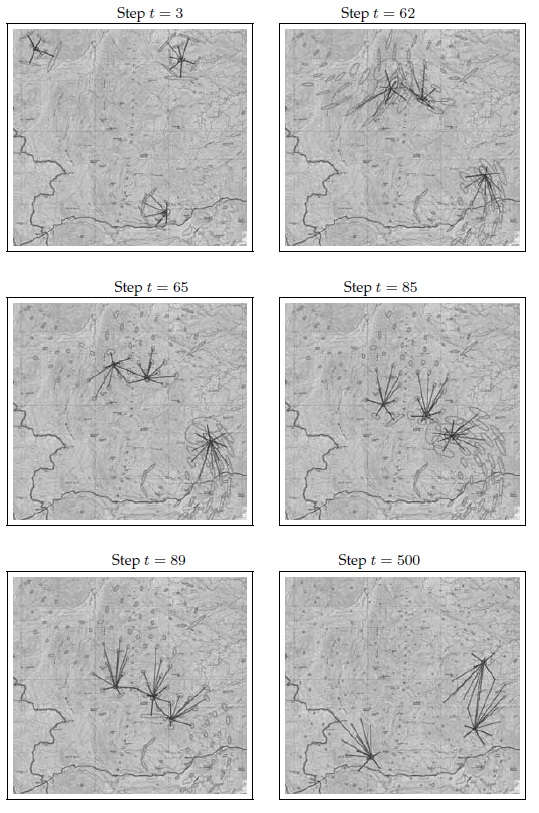
\includegraphics[width=0.95\linewidth]{1224orig}}
	\caption{ ( Рис. 12.24 Мгновенные снимки работы имитационного эксперимента SLAM в различные моменты времени. Во время выполнения шагов с 62 по 64, роботы 1 и 2 прошли через одну и ту же зону в первый раз. В результате, неопределённость их локальных карт уменьшилась. Позже, на шагах с 85 по 89, с робота 2 были обнаружены те же ориентиры, что и для транспорта 3, с похожим воздействием на общую неопределённость. После 500 шагов все ориентиры были локализованы точно. ) }
	\label{fig:1224orig}
\end{figure}

Комбинируя локальные карты на основе $m=4$ локальных признаков в таблице хэшей поиска соответствия, SEIF надёжно завершает работу, как показано на Рис. 12.23. Эта карта при вычислении через $\mu=\varOmega^{-1}\xi$, является не только суперпозицией отдельных локальных карт. Напротив, каждая локальная карта в процессе слияния слегка изменяется в результате комбинирования информации.

На Рис. 12.24 показана имитация работы трёх воздушных беспилотных аппаратов. На схеме показано, что в результате слияния карт неопределённость каждой отдельной карты уменьшилась.\\

\textbf{12.11	Выводы}\\

В этой главе описано эффективное решение проблемы онлайн SLAM – \textit{разреженный обобщенный информационный фильтр} или SEIF. SEIF похож на GraphSLAM тем, что представляет апостериорную вероятность в информационном виде. Однако, он отличается отбрасыванием прошлых положений, и может выполняться как онлайн SLAM. Было показано, что:\\

•	При отбрасывании прошлых положений признаки, обнаруженные из этих положений, приобретают прямые связи в информационной матрице.\\

•	В информационной матрице, преимущественно, находится небольшое количество связей между признаками, которые соединяют физически близко расположенные признаки. Чем дальше друг от друга расположены два признака, тем слабее связь.\\

•	Под разрежением матрицы понимается процесс смещения информации с помощью алгоритма SEIF в целях уменьшения количества связей, при этом информационная матрица всегда остаётся разреженной. Разрежённость означает, что каждый элемент матрицы соединяется ненулевым значением только с конечным множеством элементов, вне зависимости от общего размера карты $N$. Однако, разрежение является аппроксимацией, а не точной вычислительной операцией.\\

•	Было замечено, что для разреженной информационной матрицы оба шага фильтрации (измерение и обновление движения) могут быть выполнены за постоянное время, независимо от размера карты. В обычных информационных фильтрах только этап обновления измерения требует постоянного времени. Этап обновления движения требует больше времени.\\

•	Для выполнения многих шагов в SEIF все ещё требуется оценка состояния. В SEIF используется смягченный алгоритм восстановления этих оценок.\\

•	Было описано два метода ассоциации данных. Первый идентичен уже описанному для EKF SLAM - это инкрементный максимум правдоподобия. Этот метод назначает измерение наиболее вероятному признаку в каждый момент времени, но неспособен пересмотреть решение об ассоциации.\\

•	Улучшенный метод выполняет рекурсивный поиск по дереву всех ассоциаций данных, чтобы найти вектор ассоциации данных, максимизирующий правдоподобие всей совокупности данных. Это делается, используя онлайн версию алгоритма ветвей и границ с ленивым расширением дерева, когда логарифм правдоподобия данных запоминается по периметру частично расширенного дерева. Когда текущий наилучший лист достигает значения, меньшего среднему значению по периметру, периметр расширяется, пока его значение не уменьшится или же пока не будет найдено лучшее глобальное решение проблемы ассоциации данных.\\

•	Также приведено обсуждение использования SEIF в контексте картографирования с использованием нескольких роботов. Алгоритм используется в качестве внутреннего цикла метода для поворота и смещения карт, представленных в информационном виде, без необходимости вычисления самой подлежащей карты. Эта операция сохраняет разрежённость информационной матрицы.\\

•	Эскизно был приведён алгоритм, который позволяет эффективно установить глобальное соответствие между двумя картами в задаче картографирования с помощью нескольких роботов. Он создаёт хэши локальных конфигураций признаков и использует технологии быстрого поиска для установки соответствия. Затем выполняется рекурсивное слияние карт, и, если карты хорошо накладываются, то и их слияние.\\

SEIF является первым эффективным онлайновым алгоритмом SLAM описанным в книге. Он соединяет элегантность информационного выражения с идеей отбрасывания прошлых положений. Это «ленивый родственник» EKF: там, где в EKF информация каждого нового измерения активно распространяется через сеть признаков для вычисления точной общей ковариации, SEIF лишь собирает эту информацию, постепенно разрешая ее со временем. Ассоциация данных на основе дерева в SEIF также ленивая: она учитывает альтернативные пути только для наилучшего текущего пути и только при необходимости. Это строго противоположно методу, описанному в следующей главе, где  к задаче ассоциации данных применяются многочастичные фильтры. 

Для возможности эффективной работы онлайн в SEIF необходимо использовать ряд аппроксимаций, которые делают его более точным, чем GraphSLAM или EKF. В частности, у SEIF есть два ограничения: во-первых, линеаризация выполняется только однажды, так же, как в EKF. В GraphSLAM может выполняться повторная линеаризация, что, в общем, улучшает точность результата. Во-вторых, в SEIF используется аппроксимация для сохранения разрежённости информационной матрицы. Разрежённость является естественным свойством алгоритма GraphSLAM в силу природы информации, интегрирование которой выполняется при работе.

Хотя каждая из основных операций SEIF (с известным соответствием) может быть выполнена за «постоянное время», следует соблюдать осторожность. Если алгоритм SEIF применён к линейной системе (то есть нет необходимости выполнять разложение в ряд Тейлора, и ассоциация данных известна), обновление действительно займёт постоянное время. Однако, из-за необходимости линеаризации, понадобится оценить среднее $\mu_t$, а также информационное состояние. Эта оценка не поддерживается в традиционном информационном фильтре, и ее восстановление требует определённого времени. Представленная реализация SEIF только аппроксимирует ее, и качество апостериорной оценки зависит от качества этой аппроксимации.\\

\textbf{12.12	Библиографические примечания}\\

Литература по информационно-теоретическим выражениям в SLAM уже обсуждалась в предыдущей главе, в той степени, которая относится к оффлайновому представлению. Информационные фильтры имеют сравнительно короткую историю в области исследования по SLAM. В 1997 году Цорба разработал информационный фильтр, сохраняющий относительную информацию между триплетами из трёх ориентиров. Возможно, он был первым, кто заметил, что такие информационные связи косвенно сохраняют глобальную корреляцию информации, и положил начало алгоритмам с квадратичными и линейными требованиями к памяти. Ньюман (Newman, 2000), Ньюман и Дюран-Уайт (Newman and Durrant-Whyte, 2001) разработали схожий информационный фильтр, но оставили открытым вопрос о том, как именно образуются информационные связи "ориентир-ориентир". Амбициозно назвав алгоритм «целостный, сходящийся и выполняемый за постоянное время SLAM» (“consistent, convergent, and constant-time SLAM,”) Леонард и Ньюман эффективно выполнили выравнивание, успешно применив его в подводном аппарате, оснащённом сонаром с синтетической апертурой (Newman and Rikoski 2003).\\

ТОНКИЙ РАЗДЕЛИТЕЛЬНЫЙ ФИЛЬТР\\

Другой основополагающий алгоритм в этой области, это тонкий разделительный фильтр Паскина (Paskin, 2003), выражающий апостериорное распределение SLAM в виде разреженной сети, известной как тонкие разделительные деревья (Pearl 1988, Cowell et al. 1999). Та же идея была использована Фризи (Frese, 2004), который разработал древовидную факторизацию информационной матрицы для эффективного вывода.\\
ПЕРЕСЕЧЕНИЕ КОВАРИАЦИИ\\
Джулиер и Ульманн (Julier and Uhlmann) разработали масштабируемый метод под названием пересечение ковариаций (covariance intersection), выполняющий разреженную оценку апостериорного распределения таким образом, чтобы предотвратить чрезмерную степень «уверенности» алгоритма.
Их алгоритм был успешно реализован в семействе роботов NASA MARS Rover (Uhlmann et al. 1999). Перспектива информационного фильтра также относится к ранней работе Булата и Деви (Bulata and Devy, 1996), в методе которых модель ориентира сначала получалась локальных эталонных ориентиро-центрических координатах, и только затем присоединялась к целостной глобальной карте путём разрешения относительной информации между ориентирами. Наконец, некоторые «оффлайновые» алгоритмы SLAM, решающие полную задачу SLAM, такие, как были предложены Боссе (Bosse et al., 2004), Гутманом и Конолиги (Gutmann and Konolige, 2000), Фризи (Frese, 2004) и Монтемерло и Трун (Montemerlo and Thrun, 2004), оказались достаточно быстрыми для работы в режиме онлайн на ограниченных наборах данных.

Слияние карт нескольких роботов обсуждалось в работе Гутмана и Конолиги (Gutmann and Konolige, 2000). Неттлтон (Nettleton et al., 2003) был первым автором, который обобщил информационное выражение для проблемы SLAM с несколькими роботами. Они обнаружили, что аддитивность информации позволила выполнить асинхронную интеграцию локальных карт между роботами. Они также обнаружили, что добавление субкарт даёт эффективные алгоритмы связи, а интеграция карт будет выполняться за время, логарифмически зависящее от числа задействованных роботов. Однако, они не пояснили, как выравнивать эти карты, и эта проблема была позже исследована Труном и Лю (Thrun and Liu,  2003).

Алгоритм SEIF был разработан Труном (Thrun et al., 2002), и приводится в работе (Thrun et al., 2004a). По нашему мнению, это первый алгоритм, выводящий создание связей между парами признаков с точки зрения фильтрации. Жадный алгоритм ассоциации данных для SEIF был разработан Лю и Труном (Liu and Thrun, 2003), которая была впоследствии обобщена для задачи SLAM с несколькими роботами Труном и Лю (Thrun and Liu, 2003). Поиск ассоциации данных методом ветвей и границ принадлежит Хенелу (Hähnel et al., 2003a), и основывается на более ранних методах ветвей и границ, описанных Лоулером и Вудом (Lawler and Wood, 1966) и Наренда и Фукунага (Narendra and Fukunaga, 1977). Она согласуется с работой Куперса (Kuipers et al., 2004), который разработал похожий метод ассоциации данных, хотя и не в контексте информационных теоретических концепций. SEIF применялся для задач картографии заброшенных шахт (Thrun et al. 2004c), генерируя карты с $10^8$ признаков.

Набор данных парка Виктории, на который приведены ссылки в этой главе, принадлежит Гюванту (Guivant et al., 2000).\\

\textbf{12.14	Упражнения}\\

1.	Сравнить степень разрежённости в GraphSLAM и SEIF. Каковы преимущества и недостатки каждого метода? Описать условия, при которых каждый метод будет предпочтителен. Чем более конкретны аргументы, тем лучше.\\

ЦЕЛОСТНОСТЬ\\

2.	Важной концепцией многих исследователей SLAM является целостность. В сообществе SLAM целостность определяется несколько иначе, чем в общей области статистики (где целостность является асимптотическим свойством).\\

Пусть $x$ будет случайным вектором, а $\mathcal{N}(\mu,\varSigma)$ – гауссовой оценкой $x$. Гауссиан считается целостным, если соблюдаются следующие два свойства:\\

\textbf{Условие 1: Несмещённость:} Среднее $\mu$ является несмещенной\\

$$E[\mu]=x$$ 

\textbf{Условие 2: Отсутствие «самоуверенности»:} Ковариация $\varSigma$ не вызывает чрезмерной доверительности алгоритма.
Пусть $\varXi$ будет истинной ковариацией оценочной функции $\mu$:

$$\varXi=E[(\mu-E[\mu])(\mu-E[\mu])^T]$$

Тогда $\varSigma$ чрезмерно доверительна, если существует вектор $\bar{x}$, для которого\\

$$\bar{x}^T\varSigma^{-1}\bar{x}>\bar{x}^T\varXi^{-1}\bar{x}$$

Чрезмерная доверительность образуется, если 95\% эллипса доверительности оценённой ковариации $\varSigma$ попадает внутрь или пересекается с истинным эллипсом доверительности оценочной функции. 

Доказательство целостности обычно затруднено для алгоритмов SLAM. В данном случае необходимо доказать или опровергнуть, что разрежение сохраняет целостность (см. Равенство (12.20)). В частности, доказать или опровергнуть следующее предположение: \textit{для целостной объединённой вероятности $p(a, b, c)$ в гауссовой форме следующая аппроксимация также будет целостна:}\\

$$\bar{p}(a,b,c)=\frac{p(a,c)p(b,c)}{p(c)}$$

3.	Требуется реализовать алгоритм SEIF для линейного гауссового SLAM. В линейном гауссовом SLAM, уравнение движения имеет простой аддитивный вид\\

$$x_t\sim\mathcal{N}(x_{t-1}+u_t,R)$$

а уравнение измерения - вид\\

$$z_t=\mathcal{N}(m_j-x_t,Q)$$

где $R$ и $Q$ - диагональные матрицы ковариации. Ассоциация данных известна в линейных гауссовых SLAM.\\

(a)	Запустить алгоритм в простых средах имитации и проверить правильность реализации.\\

(b)	Показать на графике ошибку SEIF в виде функции разрежённости информационной матрицы. Какие выводы можно сделать?\\

(c)	Показать на графике вычислительное время для разработанной реализации SEIF в виде функции разрежённости информационной матрицы. Отметить особенности.\\

4.	Правило разрежённости в SEIF отфильтровывает все пассивные признаки $m^-$, назначая $m^-=0$. Зачем это делается? Каким будет уравнение обновления, если эти признаки не отфильтровать? Будет ли результат более или менее точным? Будет ли вычисление более или менее эффективным? Дать краткий ответ.\\

5.	В настоящее время SEIF выполняют линеаризацию сразу после интеграции команды на движение в фильтре. Обсудить возможность алгоритма SEIF, позволяющего ретроспективное изменение линеаризации. Как будет выражено апостериорное распределение такого алгоритма? Как будет выражена информационная матрица?\\










 
\end{document}